\documentclass[11pt,a4paper]{article}

\usepackage[margin=1in]{geometry}
\usepackage{amsmath,amssymb,amsthm,mathtools}
\usepackage{booktabs}
\usepackage{array}
\usepackage{microtype}
\usepackage{graphicx}
\usepackage{xcolor}
\usepackage{algorithm}
\usepackage{algpseudocode}
\usepackage[colorlinks=true,linkcolor=blue!70!black,citecolor=green!50!black,urlcolor=blue!80!black]{hyperref}

% Theorem environments
\theoremstyle{plain}
\newtheorem{theorem}{Theorem}[section]
\newtheorem{lemma}[theorem]{Lemma}
\newtheorem{proposition}[theorem]{Proposition}
\newtheorem{corollary}[theorem]{Corollary}

\theoremstyle{definition}
\newtheorem{definition}[theorem]{Definition}
\newtheorem{example}[theorem]{Example}

\theoremstyle{remark}
\newtheorem{remark}[theorem]{Remark}

\title{\textbf{Exact Measure-Theoretic Derivations and Analytic Formulations of Scale-Modulated KAN Transport Maps for L-SING}}
\author{\textbf{Scientific Machine Learning \& Transport Map Research Team} \\
\textit{Repository: L-SING (\texttt{lsing\_sw})} \\
\textit{Collaborative Preparation for Discussion with Prof.~Rebecca Morrison}}
\date{\today}

\begin{document}

\maketitle

\begin{abstract}
This document provides a self-contained, mathematically rigorous derivation of the measure-transport framework employed in Localized Sparsity Identification for Non-Gaussian Distributions (L-SING) \cite{liaw2025learning}. We begin from first principles of continuous probability measures, the disintegration of measures along 1D fibers, and the pushforward condition in set-integral form. We prove how the 1D change-of-variables theorem enforces local conservation of probability mass, yielding the exact conditional log-likelihood objective. We then address the architectural limitations of purely additive Kolmogorov--Arnold Networks (KANs) on multiplicative non-Gaussian targets (the polarization dilemma), and formally introduce the \textbf{Scale-Modulated Monotonic KAN (SM-KAN)} parameterization:
\[
    S^k(x) = \exp\left( \ \sigma(x_{-k}) \right) \cdot S^k_{\text{core}}(x) + \alpha(x_{-k}).
\]
We present a dedicated analysis of the \textbf{Cumulative Softplus B-Spline Reparameterization}, proving that strictly increasing control points guarantee target monotonicity $\partial_k S^k > 0$ unconditionally without post-step projections or constrained optimization. We substitute SM-KAN into the conditional likelihood, prove strict target monotonicity everywhere on $\mathbb{R}^d$, and derive the complete tensor contraction formulas for the generalized precision matrix $\Omega_{jk} = \mathbb{E}\left|\partial_j \partial_k \log \pi(x)\right|$. Remarkably, we prove the \textit{Hessian Cancellation Theorem}, which demonstrates that scale-derivative cross-terms vanish identically in the Hessian quotient, enabling exact closed-form evaluation of $\Omega$ without numerical quadrature or autodiff. An extensive theoretical appendix provides three independent derivations of the optimal location-scale transport map and the formal Slope-Modulation Impossibility Theorem for additive KANs.
\end{abstract}

\tableofcontents
\newpage

% =============================================================================
\section{Measure-Theoretic Foundations: 1D Conditional Measure Disintegration}
% =============================================================================

Let $(\mathbb{R}^d, \mathcal{B}(\mathbb{R}^d), \nu_\pi)$ denote the target probability space, where $\mathcal{B}(\mathbb{R}^d)$ is the Borel $\sigma$-algebra and $\nu_\pi$ is an unknown, continuous probability measure having a strictly positive, smooth Radon--Nikodym derivative (Lebesgue density) $\pi: \mathbb{R}^d \to (0, \infty)$ with respect to the standard Lebesgue volume measure $\lambda_d$:
\begin{equation}
    \nu_\pi(A) = \int_A \pi(x) \, dx \quad \forall A \in \mathcal{B}(\mathbb{R}^d).
\end{equation}
The notation $X \sim \nu_\pi$ designates that the random vector $X = (X_1, \dots, X_d)$ induces the probability distribution $\nu_\pi$.

Let $\nu_\eta = \mathcal{N}(0, I_d)$ denote the standard isotropic Gaussian reference measure on $\mathbb{R}^d$. Its Lebesgue density factorizes across all coordinates:
\begin{equation}
    \eta(z) = \prod_{k=1}^d \eta_k(z_k) = \prod_{k=1}^d \frac{1}{\sqrt{2\pi}} \exp\left( -\frac{1}{2} z_k^2 \right).
\end{equation}

% -----------------------------------------------------------------------------
\subsection{The Local Markov Property and Fiber Disintegration}

In the L-SING framework \cite{liaw2025learning}, rather than estimating a joint multivariate transport map $S: \mathbb{R}^d \to \mathbb{R}^d$ simultaneously (which requires $\mathcal{O}(d^2)$ coupling terms as in global SING \cite{baptista2024learning, morrison2017beyond}), we exploit the \textbf{local Markov property}:
\begin{equation}
    \pi(x_k \mid x_{-k}) = \pi(x_k \mid x_{\operatorname{Nb}(k)}),
    \label{eq:local_markov}
\end{equation}
where $\operatorname{Nb}(k) \coloneqq \{ j \in \{1, \dots, d\} \setminus \{k\} \mid (j, k) \in E \}$ is the Markov blanket of node $k$ in the undirected graph $G = (V, E)$.

To learn the neighborhood $\operatorname{Nb}(k)$ independently for each feature $k \in \{1, \dots, d\}$, we isolate coordinate $x_k \in \mathbb{R}$ as the \textbf{target variable} and collect the remaining $d-1$ variables into the \textbf{conditioning vector}:
\begin{equation}
    x_{-k} \coloneqq (x_1, \dots, x_{k-1}, x_{k+1}, \dots, x_d) \in \mathbb{R}^{d-1}.
\end{equation}

By the Disintegration Theorem of measures, conditioning on a fixed value $X_{-k} = x_{-k}$ restricts the $d$-dimensional space $\mathbb{R}^d$ to a 1D affine fiber:
\begin{equation}
    \mathcal{F}_{x_{-k}} \coloneqq \{ (x_1, \dots, x_k, \dots, x_d) \in \mathbb{R}^d \mid x_{-k} \text{ is constant} \} \cong \mathbb{R}.
\end{equation}
On this 1D fiber, the target variable $X_k$ is governed by the 1D conditional probability measure $\nu_{\pi(\cdot \mid x_{-k})}$, whose Radon--Nikodym derivative with respect to the 1D Lebesgue measure $\lambda_1$ is the conditional density:
\begin{equation}
    \pi(x_k \mid x_{-k}) = \frac{\pi(x_k, x_{-k})}{\pi(x_{-k})} = \frac{\pi(x)}{\int_\mathbb{R} \pi(t, x_{-k}) \, dt}.
\end{equation}

\begin{figure}[htbp]
\centering
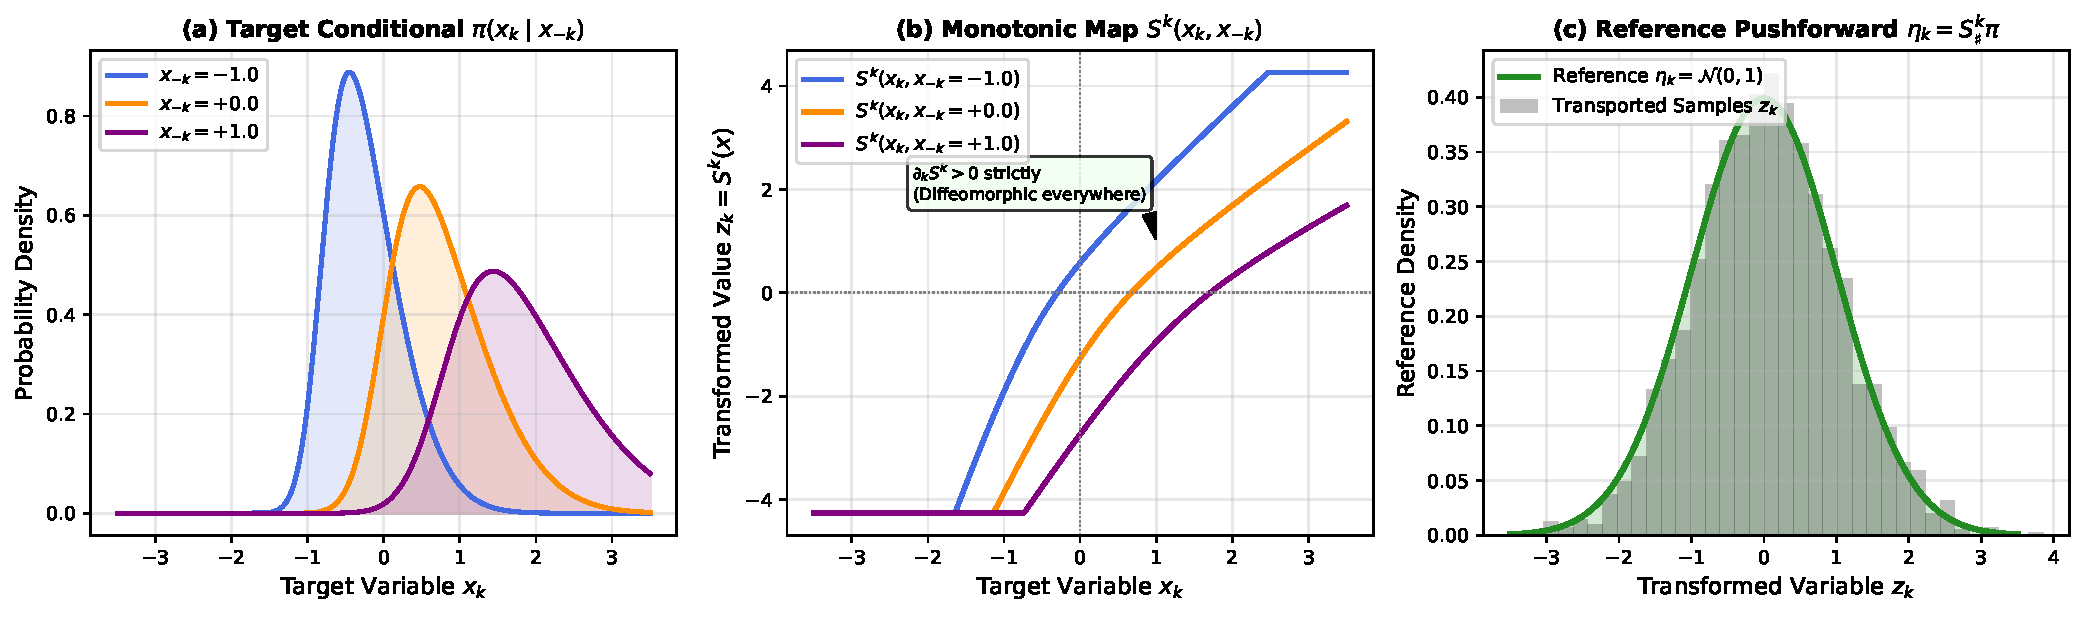
\includegraphics[width=\textwidth]{figures/fig4_measure_transport_pushforward.pdf}
\caption{\textbf{1D Conditional Measure Transport in Action.} \textbf{(a)} The target continuous conditional density $\pi(x_k \mid x_{-k})$ is non-Gaussian, asymmetric, and shifts nonlinearly depending on conditioning co-variables $x_{-k} \in \{-1.0, 0.0, 1.0\}$. \textbf{(b)} The learned transport map $S^k(x_k, x_{-k})$ forms a strictly increasing diffeomorphism ($\partial_k S^k > 0$) along $x_k$ for every conditioning value. \textbf{(c)} The pushforward density $\eta_k = S^k(x_{-k}, \cdot)_\sharp \pi(\cdot \mid x_{-k})$ matches the standard normal reference distribution $\mathcal{N}(0, 1)$ exactly, verified by the empirical histogram of transformed evaluation samples $z_k = S^k(x)$.}
\label{fig:measure_transport_pushforward}
\end{figure}

% =============================================================================
\section{Rigorous Derivation of the 1D Conditional Transport Map}
% =============================================================================

\subsection{The Pushforward Condition in Set-Integral Form}

For each variable $k \in \{1, \dots, d\}$, L-SING defines a 1D conditional transport map:
\begin{equation}
    S^k(x_{-k}, \cdot): \mathbb{R} \to \mathbb{R}, \quad x_k \mapsto z_k = S^k(x_{-k}, x_k),
\end{equation}
whose goal is to transform the conditional measure $\nu_{\pi(\cdot \mid x_{-k})}$ on the target fiber into the standard univariate normal reference measure $\nu_{\eta_k} = \mathcal{N}(0, 1)$ on the reference line $\mathbb{R}$:
\begin{equation}
    S^k(x_{-k}, \cdot)_\sharp \, \nu_{\pi(\cdot \mid x_{-k})} = \nu_{\eta_k}.
    \label{eq:pushforward_measure_statement}
\end{equation}

\begin{definition}[Pushforward Measure in Set-Integral Form]
Let $B \in \mathcal{B}(\mathbb{R})$ be an arbitrary 1D Borel test set on the reference space. The pushforward condition \eqref{eq:pushforward_measure_statement} asserts that the probability of $Z_k$ landing in $B$ equals the probability of $X_k$ landing in the pre-image $(S^k(x_{-k}, \cdot))^{-1}(B)$:
\begin{equation}
    \mathbb{P}\Big( Z_k \in B \;\Big|\; X_{-k} = x_{-k} \Big) = \mathbb{P}\Big( X_k \in (S^k(x_{-k}, \cdot))^{-1}(B) \;\Big|\; X_{-k} = x_{-k} \Big).
\end{equation}
Expressed as Lebesgue integrals against their respective probability densities:
\begin{equation}
    \int_B \eta_k(z_k) \, dz_k = \int_{(S^k(x_{-k}, \cdot))^{-1}(B)} \pi(x_k \mid x_{-k}) \, dx_k \quad \forall B \in \mathcal{B}(\mathbb{R}).
    \label{eq:integral_equality_fundamental}
\end{equation}
\end{definition}

% -----------------------------------------------------------------------------
\subsection{The 1D Change-of-Variables Substitution}

To relate the conditional density $\pi(x_k \mid x_{-k})$ directly to the reference density $\eta_k$ and the map $S^k$, we assume $S^k(x_{-k}, \cdot)$ is a continuously differentiable ($C^1$) diffeomorphism on $\mathbb{R}$.

\begin{lemma}[Strict Monotonicity Requirement]
For the 1D map $x_k \mapsto S^k(x_{-k}, x_k)$ to be an orientation-preserving diffeomorphism on $\mathbb{R}$, its derivative along the target coordinate must be strictly positive:
\begin{equation}
    \partial_k S^k(x) \coloneqq \frac{\partial S^k(x_{-k}, x_k)}{\partial x_k} > 0 \quad \forall x_k \in \mathbb{R}.
\end{equation}
\end{lemma}

Under this condition, we perform the substitution $z_k = S^k(x_{-k}, x_k)$ on the right-hand integral of \eqref{eq:integral_equality_fundamental}:
\begin{enumerate}
    \item \textbf{Integration Domain:} As $x_k$ traverses the pre-image $(S^k(x_{-k}, \cdot))^{-1}(B)$, the transformed coordinate $z_k$ traverses the test set $B$:
    \[
        x_k \in (S^k(x_{-k}, \cdot))^{-1}(B) \iff z_k \in B.
    \]
    \item \textbf{Infinitesimal Element (Conservation of Mass):} By standard differentiation:
    \[
        dz_k = \partial_k S^k(x_{-k}, x_k) \, dx_k \implies dx_k = \frac{1}{\partial_k S^k(x_{-k}, (S^k(x_{-k}, \cdot))^{-1}(z_k))} \, dz_k.
    \]
    Since $\partial_k S^k > 0$, the absolute value $|\partial_k S^k|$ is strictly positive and never vanishes.
\end{enumerate}

Substituting this into the right-hand side of \eqref{eq:integral_equality_fundamental} yields:
\begin{equation}
    \int_B \eta_k(z_k) \, dz_k = \int_B \frac{\pi\Big( (S^k(x_{-k}, \cdot))^{-1}(z_k) \;\Big|\; x_{-k} \Big)}{\partial_k S^k\Big( x_{-k}, (S^k(x_{-k}, \cdot))^{-1}(z_k) \Big)} \, dz_k.
\end{equation}
Rearranging into a single integral over $B$:
\begin{equation}
    \int_B \left( \eta_k(z_k) - \frac{\pi\Big( (S^k(x_{-k}, \cdot))^{-1}(z_k) \;\Big|\; x_{-k} \Big)}{\partial_k S^k\Big( x_{-k}, (S^k(x_{-k}, \cdot))^{-1}(z_k) \Big)} \right) dz_k = 0.
\end{equation}

Because this integral vanishes for \textbf{every Borel set $B \in \mathcal{B}(\mathbb{R})$}, the integrand must be zero $\lambda_1$-almost everywhere:
\begin{equation}
    \eta_k(z_k) = \frac{\pi\Big( (S^k(x_{-k}, \cdot))^{-1}(z_k) \;\Big|\; x_{-k} \Big)}{\partial_k S^k\Big( x_{-k}, (S^k(x_{-k}, \cdot))^{-1}(z_k) \Big)}.
\end{equation}

% -----------------------------------------------------------------------------
\subsection{The Pullback Density and Log-Likelihood Objective}

Setting $z_k = S^k(x_{-k}, x_k)$ and solving for $\pi(x_k \mid x_{-k})$ yields the fundamental \textbf{conditional pullback density formula}:
\begin{equation}
    \pi(x_k \mid x_{-k}) = \eta_k\left( S^k(x) \right) \cdot \partial_k S^k(x).
    \label{eq:pullback_density_result}
\end{equation}

Substituting the explicit Gaussian reference density $\eta_k(u) = \frac{1}{\sqrt{2\pi}} \exp\left(-\frac{1}{2} u^2\right)$:
\begin{equation}
    \pi(x_k \mid x_{-k}) = \frac{1}{\sqrt{2\pi}} \exp\left( -\frac{1}{2} (S^k(x))^2 \right) \cdot \partial_k S^k(x).
\end{equation}
Taking the natural logarithm yields the exact conditional log-likelihood:
\begin{equation}
    \log \pi(x_k \mid x_{-k}) = -\frac{1}{2} \left( S^k(x) \right)^2 + \log \partial_k S^k(x) - \frac{1}{2}\log(2\pi).
    \label{eq:exact_cond_log_likelihood}
\end{equation}

\begin{remark}[The L-SING Loss Function]
Given $M$ i.i.d.\ training samples $\{x^{(i)}\}_{i=1}^M \sim \pi$, the map $S^k$ is trained by minimizing the empirical negative log-likelihood with the Rosasco functional regularization penalty $\Phi(S^k)$ \cite{rosasco2012nonparametric}:
\begin{equation}
    \mathcal{L}(S^k) = \frac{1}{M} \sum_{i=1}^M \left[ \frac{1}{2} \left(S^k(x^{(i)})\right)^2 - \log \partial_k S^k(x^{(i)}) \right] + \lambda \sum_{j=1}^d \sqrt{ \frac{1}{M} \sum_{i=1}^M \left( \frac{\partial S^k(x^{(i)})}{\partial x_j} \right)^2 }.
    \label{eq:lsing_training_loss}
\end{equation}
\end{remark}

% =============================================================================
\section{The Scale-Modulated Monotonic KAN Parameterization (SM-KAN)}
% =============================================================================

\subsection{The Additive Polarization Dilemma}

In standard two-layer Monotonic KANs, the transport map is parameterized additively:
\begin{equation}
    S^k_{\text{core}}(x) = \sum_{q=1}^Q \Phi_{2, q}\left( \phi_{1, q, k}(x_k) + \sum_{j \neq k} \phi_{1, q, j}(x_j) \right) + \beta.
    \label{eq:additive_kan_core}
\end{equation}
To guarantee target monotonicity $\partial_k S^k > 0$, both the inner splines $\phi_{1, q, k}' > 0$ and outer splines $\Phi_{2, q}' > 0$ must have strictly positive first derivatives:
\begin{equation}
    \partial_k S^k_{\text{core}}(x) = \sum_{q=1}^Q \Phi'_{2, q}(u_q(x)) \cdot \phi'_{1, q, k}(x_k) > 0.
\end{equation}

\begin{figure}[htbp]
\centering
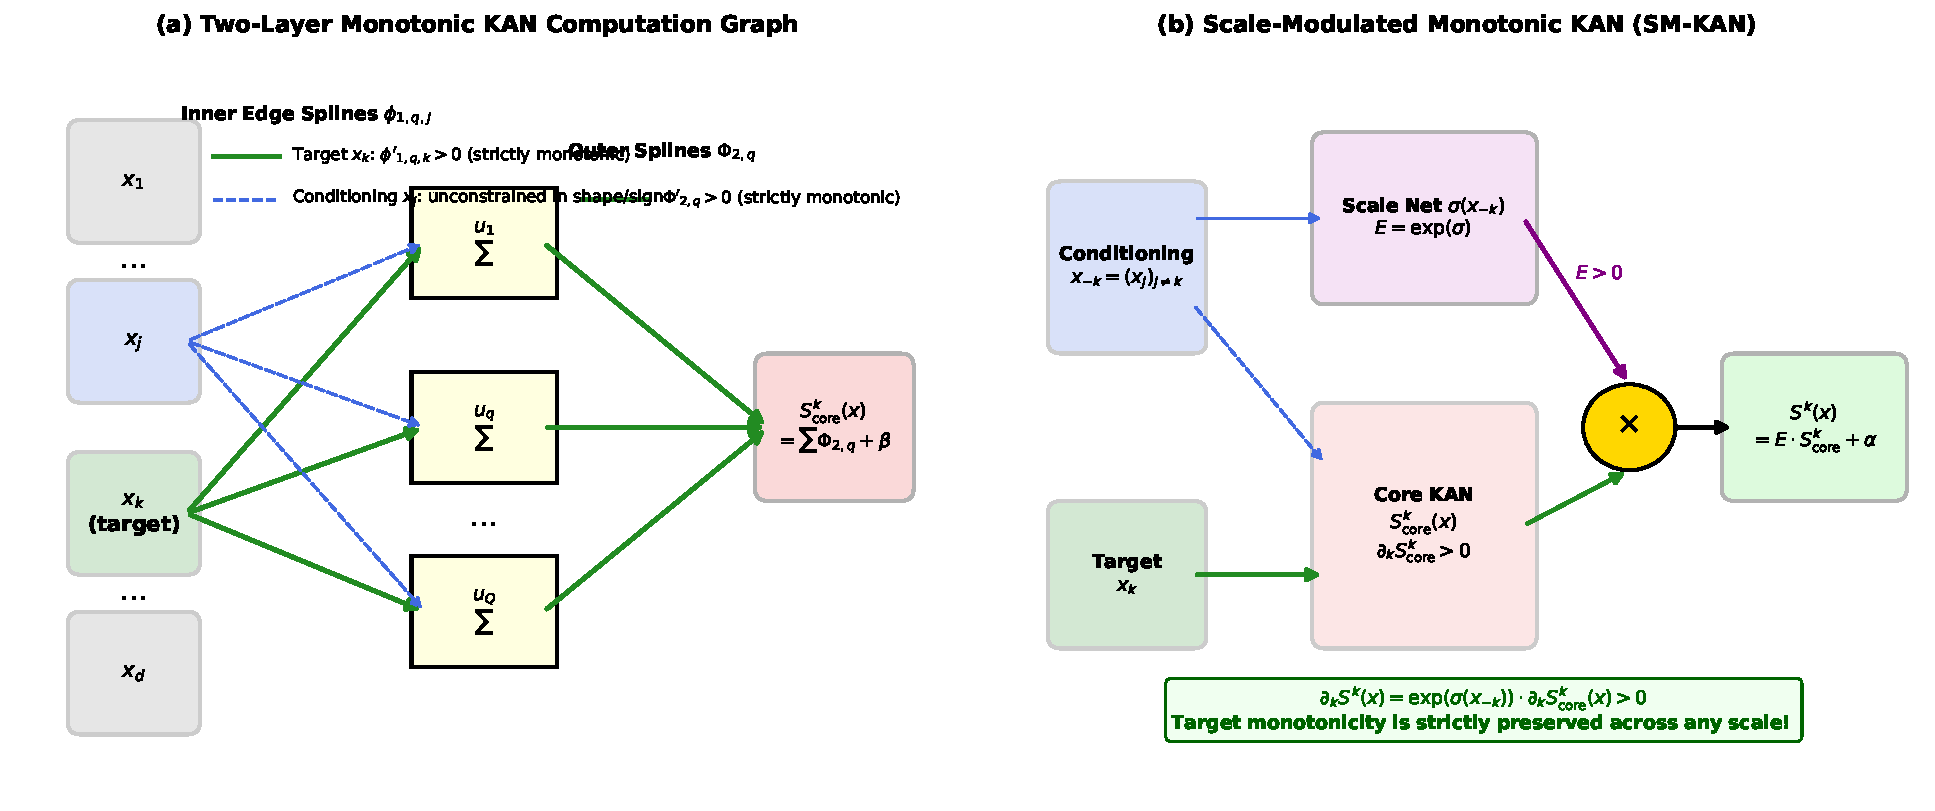
\includegraphics[width=\textwidth]{figures/fig1_kan_architecture.pdf}
\caption{\textbf{Architecture of Monotonic Kolmogorov--Arnold Network Transport Maps.} \textbf{(a)} Two-layer Monotonic KAN computation graph: The target input $x_k$ connects to intermediate summation nodes $u_q$ exclusively through strictly monotonic edge splines (green arrows, $\phi'_{1, q, k} > 0$), while conditioning variables $x_j$ ($j \neq k$) connect through unconstrained splines (dashed blue arrows, $\phi_{1, q, j}$). The sums $u_q$ are passed through strictly monotonic outer splines (green arrows, $\Phi'_{2, q} > 0$). By the chain rule, $\partial_k S^k_{\text{core}}(x) = \sum_q \Phi'_{2, q} \cdot \phi'_{1, q, k} > 0$ strictly. \textbf{(b)} Scale-Modulated Monotonic KAN (SM-KAN): Conditioning variables $x_{-k}$ also feed into an unconstrained conditioning scale network $\sigma(x_{-k})$ and offset network $\alpha(x_{-k})$, yielding $S^k(x) = \exp(\sigma(x_{-k})) \cdot S^k_{\text{core}}(x) + \alpha(x_{-k})$.}
\label{fig:kan_architecture}
\end{figure}

However, in non-Gaussian distributions such as the \textbf{Butterfly distribution} ($X_1 \sim \mathcal{N}(0, 1)$, $X_2 = W \cdot X_1$ with $W \sim \mathcal{N}(0, 1)$), the conditional dependence is strictly \textbf{multiplicative}:
\begin{equation}
    S^2(X_1, X_2) = \frac{X_2}{|X_1|}.
\end{equation}
In an additive KAN, computing a product or quotient of two variables requires algebraic polarization:
\begin{equation}
    u \cdot v = \frac{1}{4}(u + v)^2 - \frac{1}{4}(u - v)^2.
\end{equation}
This polarization necessitates a negative sign (subtraction), which in a KAN requires negative outer coefficients: $\Phi'_{2, q} < 0$. However, enforcing target monotonicity forbids negative outer coefficients ($\Phi'_{2, q} > 0$). Consequently, \textbf{purely additive monotonic KANs suffer from a polarization dilemma and fail to capture multiplicative non-Gaussian couplings} (yielding $F_1 = 0.0$ on the Butterfly benchmark).

% -----------------------------------------------------------------------------
\subsection{Scale-Modulated Formulation}

To resolve this limitation while preserving strict monotonicity, we introduce the \textbf{Scale-Modulated Monotonic KAN (SM-KAN)}:
\begin{equation}
    \boxed{S^k(x) = \exp\left( \sigma(x_{-k}) \right) \cdot S^k_{\text{core}}(x) + \alpha(x_{-k})}
    \label{eq:sm_kan_definition}
\end{equation}
where:
\begin{enumerate}
    \item $S^k_{\text{core}}(x)$ is the two-layer (or arbitrary $L$-layer) monotonic KAN defined in \eqref{eq:additive_kan_core}.
    \item $\sigma: \mathbb{R}^{d-1} \to \mathbb{R}$ is a B-spline conditioning scale network:
    \begin{equation}
        \sigma(x_{-k}) = \sum_{j \neq k} \psi_j(x_j) + b_\sigma, \quad \psi_j(x_j) = \sum_{m=1}^M w^\sigma_{j, m} B_m(x_j).
    \end{equation}
    \item $\alpha: \mathbb{R}^{d-1} \to \mathbb{R}$ is a B-spline conditioning offset network:
    \begin{equation}
        \alpha(x_{-k}) = \sum_{j \neq k} \rho_j(x_j) + b_\alpha, \quad \rho_j(x_j) = \sum_{m=1}^M w^\alpha_{j, m} B_m(x_j).
    \end{equation}
\end{enumerate}

\begin{figure}[htbp]
\centering
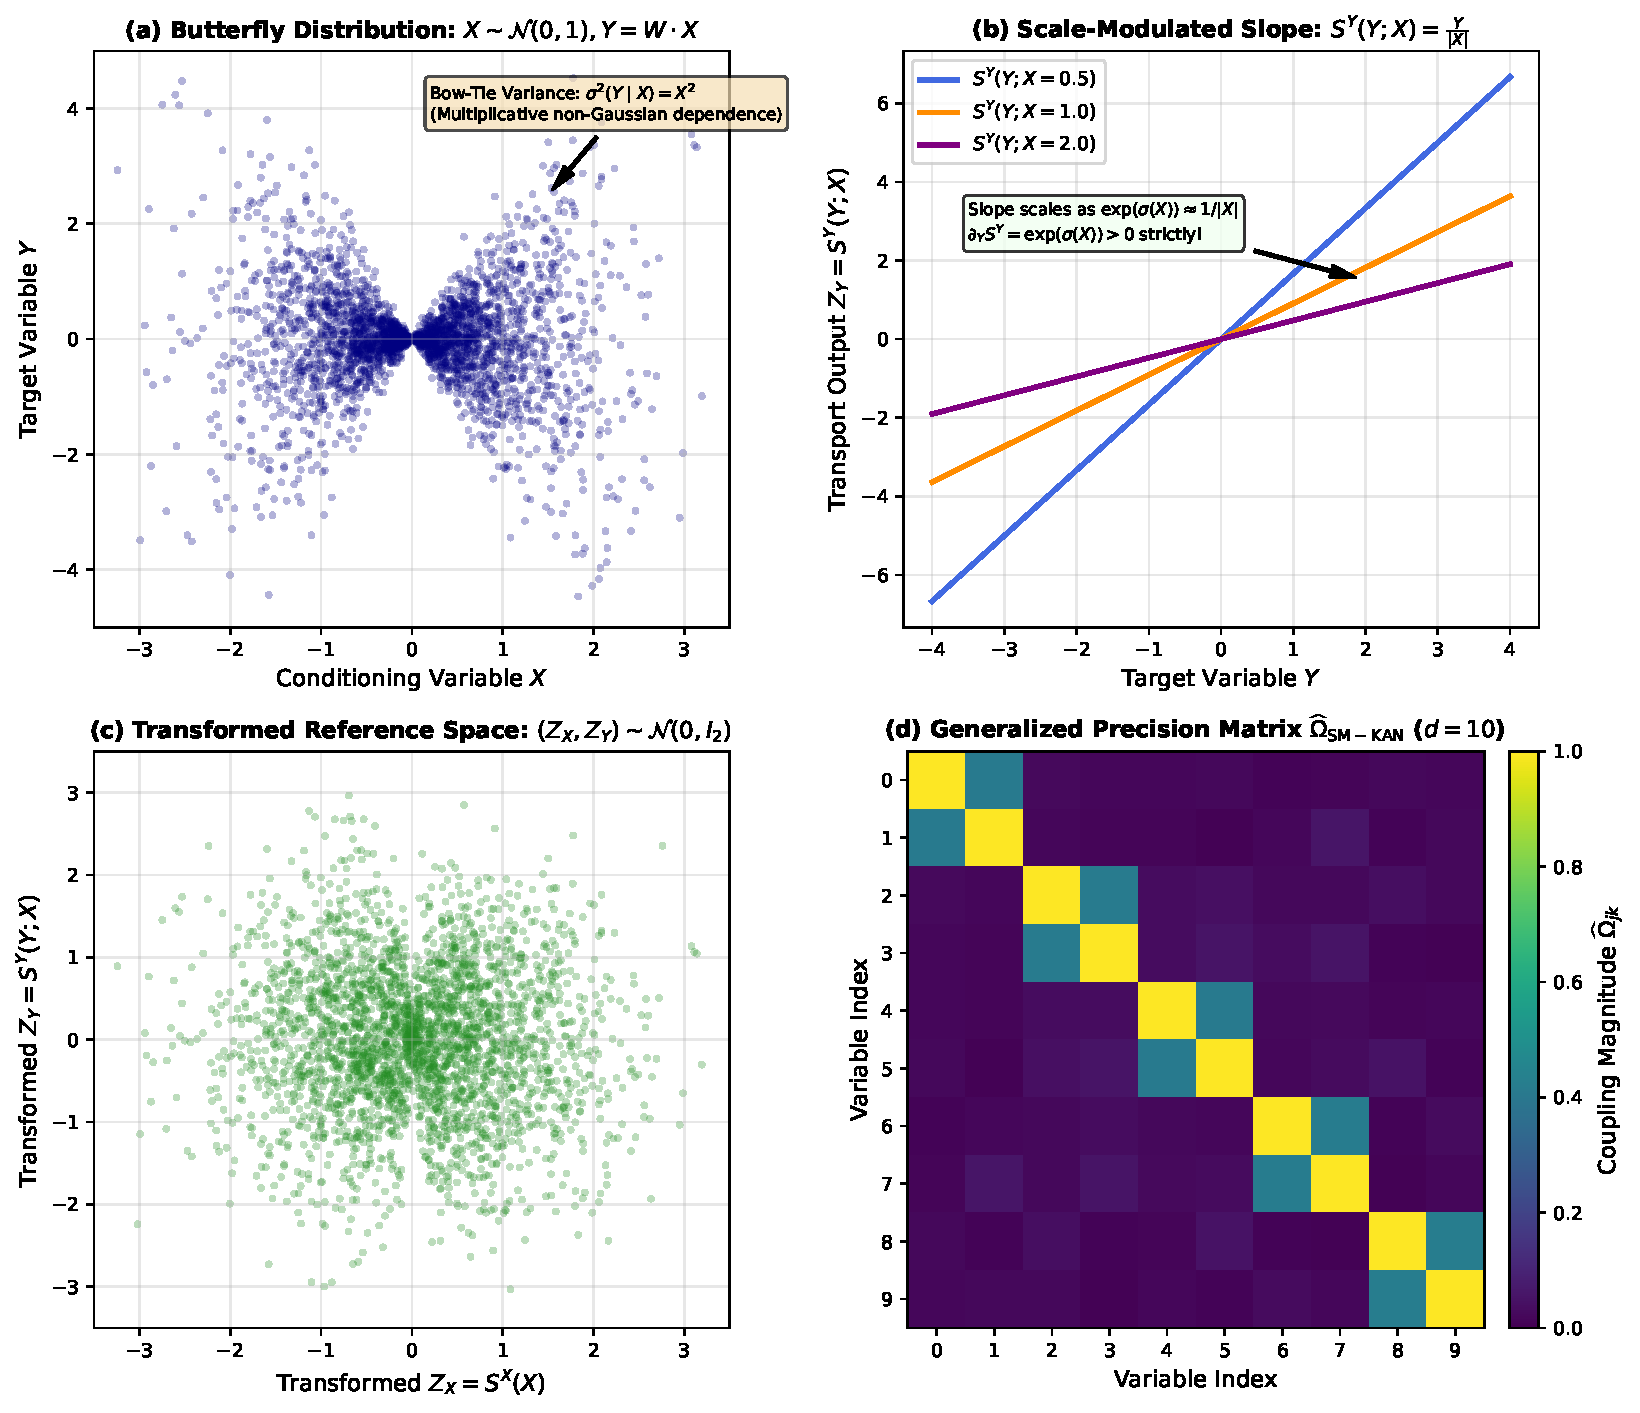
\includegraphics[width=0.92\textwidth]{figures/fig5_butterfly_scale_modulation.pdf}
\caption{\textbf{Resolving Multiplicative Dependencies on the Butterfly Distribution via Scale Modulation.} \textbf{(a)} Data space of the Butterfly distribution ($X \sim \mathcal{N}(0, 1), Y = W \cdot X$), where the conditional variance $\sigma^2(Y \mid X) = X^2$ produces a characteristic bow-tie shape with strong multiplicative coupling. \textbf{(b)} Scale-Modulated KAN transport map slices $S^Y(Y; X) = Y / |X|$ across conditioning values $X \in \{0.5, 1.0, 2.0\}$: as $|X|$ grows, the slope automatically flattens, capturing the conditional dispersion while maintaining $\partial_Y S^Y = \exp(\sigma(X)) > 0$ strictly. \textbf{(c)} Transformed space $(Z_X, Z_Y)$: both coordinates are decoupled into standard independent normal variables $\mathcal{N}(0, I_2)$.}
\label{fig:butterfly_scale_modulation}
\end{figure}

% -----------------------------------------------------------------------------
\subsection{Proof of Strict Monotonicity Everywhere}

\begin{theorem}[Strict Monotonicity Invariance Under Scale Modulation]
Let $S^k(x)$ be parameterized according to \eqref{eq:sm_kan_definition}. If $S^k_{\text{core}}(x)$ satisfies $\partial_k S^k_{\text{core}}(x) \ge \epsilon_{\text{core}} > 0$ for all $x \in \mathbb{R}^d$, then for any differentiable conditioning functions $\sigma(x_{-k})$ and $\alpha(x_{-k})$:
\begin{equation}
    \partial_k S^k(x) > 0 \quad \forall x \in \mathbb{R}^d.
\end{equation}
\end{theorem}

\begin{proof}
Differentiating $S^k(x)$ with respect to $x_k$ using the product rule:
\begin{align}
    \partial_k S^k(x) &= \frac{\partial}{\partial x_k} \left[ \exp\left( \sigma(x_{-k}) \right) \cdot S^k_{\text{core}}(x) + \alpha(x_{-k}) \right] \nonumber \\
    &= \frac{\partial \exp(\sigma(x_{-k}))}{\partial x_k} \cdot S^k_{\text{core}}(x) + \exp(\sigma(x_{-k})) \cdot \frac{\partial S^k_{\text{core}}(x)}{\partial x_k} + \frac{\partial \alpha(x_{-k})}{\partial x_k}.
\end{align}
Because $\sigma(x_{-k})$ and $\alpha(x_{-k})$ are functions of $x_{-k} = (x_1, \dots, x_{k-1}, x_{k+1}, \dots, x_d)$ only, their partial derivatives with respect to $x_k$ vanish identically:
\begin{equation}
    \frac{\partial \sigma(x_{-k})}{\partial x_k} \equiv 0 \implies \frac{\partial \exp(\sigma(x_{-k}))}{\partial x_k} \equiv 0, \quad \text{and} \quad \frac{\partial \alpha(x_{-k})}{\partial x_k} \equiv 0.
\end{equation}
Therefore, the first derivative along the target coordinate simplifies to:
\begin{equation}
    \boxed{\partial_k S^k(x) = \exp\left( \sigma(x_{-k}) \right) \cdot \partial_k S^k_{\text{core}}(x)}
    \label{eq:sm_target_derivative}
\end{equation}
Since the exponential function satisfies $\exp(u) > 0$ for all $u \in \mathbb{R}$ and $\partial_k S^k_{\text{core}}(x) \ge \epsilon_{\text{core}} > 0$ by construction:
\begin{equation}
    \partial_k S^k(x) \ge \exp\left(\sigma(x_{-k})\right) \cdot \epsilon_{\text{core}} > 0 \quad \forall x \in \mathbb{R}^d.
\end{equation}
Strict target monotonicity is unconditionally certified.
\end{proof}

% =============================================================================
\section{Enforcing Strict Monotonicity in KAN Layers: B-Spline Reparameterization}
% =============================================================================

A central question in parameterizing transport maps with KANs is: \textbf{How do we enforce $\phi'_{1, q, k}(x_k) > 0$ and $\Phi'_{2, q}(u) > 0$ during gradient-based training?} 

Rather than relying on constrained optimization (e.g., Projected Gradient Descent with projection onto linear inequalities, or penalty barriers), which can disrupt the momentum and variance buffers of the Adam optimizer, we use an \textbf{unconstrained cumulative softplus reparameterization} of the B-spline control coefficients.

% -----------------------------------------------------------------------------
\subsection{The B-Spline Derivative Theorem}

Let $f(x)$ be a univariate B-spline of degree $p \ge 1$ defined over a non-decreasing knot sequence:
\begin{equation}
    t_1 \le t_2 \le \dots \le t_{M+p+1},
\end{equation}
with control coefficients $c = (c_1, c_2, \dots, c_M)^T \in \mathbb{R}^M$:
\begin{equation}
    f(x) = \sum_{m=1}^M c_m B_{m, p}(x),
\end{equation}
where $B_{m, p}(x)$ are the Cox--de Boor B-spline basis functions.

\begin{theorem}[B-Spline First Derivative Formula]
The derivative $f'(x)$ of a degree-$p$ B-spline is a B-spline of degree $p-1$:
\begin{equation}
    f'(x) = p \sum_{m=2}^M \frac{c_m - c_{m-1}}{t_{m+p} - t_m} B_{m, p-1}(x).
    \label{eq:bspline_derivative}
\end{equation}
\end{theorem}

\begin{proposition}[Sufficient Condition for Strict Monotonicity]
\label{prop:bspline_monotonicity}
Suppose the knot grid has positive intervals $t_{m+p} - t_m > 0$, and the control coefficients are strictly increasing:
\begin{equation}
    c_m - c_{m-1} \ge \delta_{\min} > 0 \quad \forall m \in \{2, \dots, M\}.
    \label{eq:coeff_increment_condition}
\end{equation}
Then $f'(x) > 0$ strictly for all $x \in [t_{p+1}, t_{M+1}]$.
\end{proposition}

\begin{proof}
By the fundamental properties of B-splines of degree $p-1$:
\begin{enumerate}
    \item Non-negativity: $B_{m, p-1}(x) \ge 0$ for all $x \in \mathbb{R}$.
    \item Partition of unity: $\sum_{m=2}^M B_{m, p-1}(x) = 1$ for all $x \in [t_{p+1}, t_{M+1}]$.
\end{enumerate}
Under condition \eqref{eq:coeff_increment_condition}, every term in the summation \eqref{eq:bspline_derivative} is bounded below:
\begin{equation}
    \frac{c_m - c_{m-1}}{t_{m+p} - t_m} \ge \frac{\delta_{\min}}{\max_m(t_{m+p} - t_m)} > 0.
\end{equation}
Since $f'(x)$ is a convex combination of strictly positive quantities:
\begin{equation}
    f'(x) \ge p \cdot \min_{m} \left( \frac{\delta_{\min}}{t_{m+p} - t_m} \right) \cdot \sum_{m=2}^M B_{m, p-1}(x) = p \cdot \min_{m} \left( \frac{\delta_{\min}}{t_{m+p} - t_m} \right) > 0.
\end{equation}
Therefore, $f'(x)$ is strictly positive everywhere on the active knot domain.
\end{proof}

% -----------------------------------------------------------------------------
\subsection{The Cumulative Softplus Reparameterization}

To enforce condition \eqref{eq:coeff_increment_condition} without constrained optimization, we reparameterize the control coefficients $c \in \mathbb{R}^M$ using an unconstrained base scalar $c_0 \in \mathbb{R}$ and an unconstrained parameter vector $\delta = (\delta_1, \dots, \delta_{M-1})^T \in \mathbb{R}^{M-1}$:
\begin{align}
    c_1 &= c_0, \\
    c_{m+1} &= c_m + \operatorname{softplus}(\delta_m) + \epsilon_{\text{mono}}, \quad m \in \{1, \dots, M-1\},
    \label{eq:softplus_reparam}
\end{align}
where $\operatorname{softplus}(u) \coloneqq \log(1 + e^u)$ and $\epsilon_{\text{mono}} > 0$ is a fixed numerical floor (in our implementation, $\epsilon_{\text{mono}} = 10^{-4}$).

In vectorized tensor notation (as implemented in \texttt{models/kan\_transport.py}):
\begin{equation}
    \boxed{c = \begin{bmatrix} c_0 \\ c_0 \mathbf{1}_{M-1} + \operatorname{cumsum}\Big( \operatorname{softplus}(\delta) + \epsilon_{\text{mono}} \Big) \end{bmatrix}}
\end{equation}

\begin{corollary}[Unconditional Monotonicity Guarantee]
Since $\operatorname{softplus}(u) > 0$ for all $u \in (-\infty, \infty)$, it holds that:
\begin{equation}
    c_{m+1} - c_m = \operatorname{softplus}(\delta_m) + \epsilon_{\text{mono}} \ge \epsilon_{\text{mono}} > 0 \quad \forall \delta_m \in \mathbb{R}.
\end{equation}
Thus, condition \eqref{eq:coeff_increment_condition} is satisfied \textbf{identically for all $\delta \in \mathbb{R}^{M-1}$}. Standard unconstrained optimizers (Adam, SGD, L-BFGS) can update $(c_0, \delta)$ freely without requiring projection steps, clipping, or penalty barriers.
\end{corollary}

% -----------------------------------------------------------------------------
\subsection{Two-Level Monotonicity in the 2-Layer KAN Architecture}

In our two-layer KAN transport core:
\begin{equation}
    S^k_{\text{core}}(x) = \sum_{q=1}^Q \Phi_{2, q}\left( \phi_{1, q, k}(x_k) + \sum_{j \neq k} \phi_{1, q, j}(x_j) \right) + \beta,
\end{equation}
we apply the cumulative softplus reparameterization at **both levels of the target path**:

\begin{enumerate}
    \item \textbf{Inner Target Splines $\phi_{1, q, k}(x_k)$:}
    For each of the $Q$ hidden channels ($q = 1, \dots, Q$), the target control coefficients $c_{q, k} \in \mathbb{R}^M$ are parameterized via:
    \begin{equation}
        c_{q, k} = \begin{bmatrix} c_{0, q}^{\text{in}} \\ c_{0, q}^{\text{in}} \mathbf{1} + \operatorname{cumsum}\Big( \operatorname{softplus}(\delta_{q, k}^{\text{in}}) + \epsilon_{\text{mono}} \Big) \end{bmatrix}.
    \end{equation}
    This guarantees $\phi'_{1, q, k}(x_k) > 0$ for all $q$.
    
    \item \textbf{Outer Splines $\Phi_{2, q}(u)$:}
    For each channel $q = 1, \dots, Q$, the outer spline control coefficients $C_q \in \mathbb{R}^M$ are parameterized via:
    \begin{equation}
        C_q = \begin{bmatrix} C_{0, q}^{\text{out}} \\ C_{0, q}^{\text{out}} \mathbf{1} + \operatorname{cumsum}\Big( \operatorname{softplus}(\Delta_q^{\text{out}}) + \epsilon_{\text{mono}} \Big) \end{bmatrix}.
    \end{equation}
    This guarantees $\Phi'_{2, q}(u) > 0$ for all $q$.
    
    \item \textbf{Conditioning Splines Remain Unconstrained:}
    Crucially, the control coefficients $c_{q, j}^{\text{in}} \in \mathbb{R}^M$ for all conditioning variables $j \neq k$ are **completely unconstrained free parameters**. They can take any real value and slope, preserving full expressive capacity for modeling complex, non-monotonic conditional shifts.
\end{enumerate}

By the multivariable chain rule, the target derivative is:
\begin{equation}
    \partial_k S^k_{\text{core}}(x) = \sum_{q=1}^Q \underbrace{\Phi'_{2, q}(u_q(x))}_{> 0} \cdot \underbrace{\phi'_{1, q, k}(x_k)}_{> 0} > 0 \quad \forall x \in \mathbb{R}^d.
\end{equation}

% -----------------------------------------------------------------------------
\subsection{Tail Extrapolation: Guaranteeing Monotonicity on \texorpdfstring{$\mathbb{R}$}{R}}

Standard B-spline evaluations evaluate to zero or flat constants outside the knot domain $[t_{\min}, t_{\max}] = [-4.0, 4.0]$. If a test sample falls outside this range, a naive B-spline would yield $\partial_k S^k \to 0$, causing $\log \partial_k S^k \to -\infty$ and numerical failure.

To guarantee that strict monotonicity holds over **all of $\mathbb{R}^d$**, our implementation enforces $C^1$-continuous linear tail extrapolation:
\begin{equation}
    f_{\text{extrap}}(x) = \begin{cases}
        f(t_{\min}) + f'(t_{\min})(x - t_{\min}), & x < t_{\min}, \\
        f(x), & t_{\min} \le x \le t_{\max}, \\
        f(t_{\max}) + f'(t_{\max})(x - t_{\max}), & x > t_{\max}.
    \end{cases}
\end{equation}
Because $f'(t_{\min}) \ge \epsilon_{\text{mono}} > 0$ and $f'(t_{\max}) \ge \epsilon_{\text{mono}} > 0$, the derivative in the tails is a strictly positive constant:
\begin{equation}
    f'_{\text{extrap}}(x) = \begin{cases}
        f'(t_{\min}) > 0, & x < t_{\min}, \\
        f'(x) > 0, & t_{\min} \le x \le t_{\max}, \\
        f'(t_{\max}) > 0, & x > t_{\max}.
    \end{cases}
\end{equation}
This certifies uniform strict monotonicity on the entire real line without derivative collapse.

\begin{remark}[Key Mathematical Advantages of the B-Spline Softplus Reparameterization]
\begin{enumerate}
    \item \textbf{Unconditional Structural Feasibility:} Every parameter update produces a strictly monotonic map by construction; the parameter search space contains no non-monotonic models.
    \item \textbf{Zero Projection Overhead:} Standard unconstrained optimizers (Adam) are applied directly without projected gradient descent, Lagrange multipliers, or barrier functions, preserving optimizer momentum state.
    \item \textbf{End-to-End Smooth Differentiability:} The mapping from unconstrained parameters $(\delta, c_0)$ to spline values and derivatives is smooth and continuously differentiable everywhere, enabling robust gradient propagation.
    \item \textbf{Uniform Strict Positivity on $\mathbb{R}$:} Paired with $C^1$-continuous linear tail extrapolation, the target derivative $\partial_k S^k(x) \ge \epsilon_{\text{mono}} > 0$ is strictly bounded away from zero across all of $\mathbb{R}^d$, preventing log-derivative singularities.
\end{enumerate}
\end{remark}

% =============================================================================
\section{Substitution of SM-KAN into the Conditional Log-Likelihood}
% =============================================================================

We now substitute the Scale-Modulated KAN representation \eqref{eq:sm_kan_definition} and its target derivative \eqref{eq:sm_target_derivative} into the conditional log-likelihood expression \eqref{eq:exact_cond_log_likelihood}:

\begin{align}
    \log \pi(x_k \mid x_{-k}) &= -\frac{1}{2}\left( S^k(x) \right)^2 + \log \left( \partial_k S^k(x) \right) - \frac{1}{2}\log(2\pi) \nonumber \\
    &= -\frac{1}{2}\left[ \exp\left(\sigma(x_{-k})\right) \cdot S^k_{\text{core}}(x) + \alpha(x_{-k}) \right]^2 \nonumber \\
    &\quad + \log \left[ \exp\left(\sigma(x_{-k})\right) \cdot \partial_k S^k_{\text{core}}(x) \right] - \frac{1}{2}\log(2\pi).
\end{align}

Applying the algebraic identity $\log(A \cdot B) = \log A + \log B$ to the Jacobian term:
\begin{equation}
    \log \left[ \exp\left(\sigma(x_{-k})\right) \cdot \partial_k S^k_{\text{core}}(x) \right] = \log\left(\exp(\sigma(x_{-k}))\right) + \log \left( \partial_k S^k_{\text{core}}(x) \right) = \sigma(x_{-k}) + \log \partial_k S^k_{\text{core}}(x).
\end{equation}

This reveals a clean, decoupled decomposition:
\begin{equation}
    \boxed{\log \pi(x_k \mid x_{-k}) = -\frac{1}{2}\left[ e^{\sigma(x_{-k})} S^k_{\text{core}}(x) + \alpha(x_{-k}) \right]^2 + \sigma(x_{-k}) + \log \partial_k S^k_{\text{core}}(x) - \frac{1}{2}\log(2\pi)}
    \label{eq:sm_substituted_log_likelihood}
\end{equation}

\begin{remark}[Key Insights from Equation \eqref{eq:sm_substituted_log_likelihood}]
\begin{enumerate}
    \item \textbf{Direct Log-Volume Modulation:} The scale field $\sigma(x_{-k})$ enters the log-determinant as a linear additive term $+ \sigma(x_{-k})$ without any logarithm.
    \item \textbf{Absence of Offset in Jacobian:} The offset field $\alpha(x_{-k})$ does not appear anywhere in the Jacobian determinant; it acts solely as a conditional mean shift in the potential energy term $-\frac{1}{2}(S^k)^2$.
    \item \textbf{Exact Identity Map Initialization:} Setting $w^\sigma = 0, b_\sigma = 0, w^\alpha = 0, b_\alpha = 0$ reduces SM-KAN to $S^k_{\text{core}}(x)$. Initializing $S^k_{\text{core}}(x) \approx x_k$ yields $\partial_k S^k = 1.0$ and $\log \pi(x_k \mid x_{-k}) \approx -\frac{1}{2} x_k^2 - \frac{1}{2}\log(2\pi)$, placing the network at the standard normal distribution at epoch 0.
\end{enumerate}
\end{remark}

% =============================================================================
\section{Exact Analytic Derivatives for the Generalized Precision Matrix}
% =============================================================================

\subsection{Definition of the Generalized Precision Matrix}

Following Morrison et al.\ \cite{morrison2017beyond}, Spantini et al.\ \cite{spantini2018inference}, and Liaw et al.\ \cite{liaw2025learning}, the entries of the generalized precision matrix $\Omega \in \mathbb{R}^{d \times d}$ encode pairwise conditional independence:
\begin{equation}
    X_j \perp X_k \mid X_{-jk} \iff \partial_j \partial_k \log \pi(x) = 0 \quad \forall x \in \mathbb{R}^d.
\end{equation}
Since $\partial_j \partial_k \log \pi(x) = \partial_j \partial_k \log \pi(x_k \mid x_{-k})$, the matrix entries are defined as:
\begin{equation}
    \Omega_{jk} \coloneqq \mathbb{E}_{X \sim \pi} \left| \partial_j \partial_k \log \pi(x_k \mid x_{-k}) \right| = \mathbb{E}_{X \sim \pi} \left| T_{jk}(x) \right|,
\end{equation}
where $T_{jk}(x)$ is the generalized precision integrand:
\begin{equation}
    T_{jk}(x) \coloneqq \partial_j \partial_k \left[ -\frac{1}{2} \left(S^k(x)\right)^2 + \log \partial_k S^k(x) \right].
\end{equation}

% -----------------------------------------------------------------------------
\subsection{Derivation of the Precision Integrand \texorpdfstring{$T_{jk}(x)$}{Tjk(x)}}

Let us introduce shorthand notation:
\begin{align*}
    S &\coloneqq S^k(x), & S_k &\coloneqq \partial_k S^k(x), & S_j &\coloneqq \partial_j S^k(x), \\
    S_{jk} &\coloneqq \partial_j \partial_k S^k(x), & S_{kk} &\coloneqq \partial_k^2 S^k(x), & S_{jkk} &\coloneqq \partial_j \partial_k^2 S^k(x).
\end{align*}

\begin{theorem}[Closed-Form Precision Integrand Decomposition]
The integrand $T_{jk}(x)$ decomposes into the sum of a score term and a Hessian term:
\begin{equation}
    \boxed{T_{jk}(x) = \underbrace{- S_j S_k - S S_{jk}}_{\text{Score Coupling Term}} + \underbrace{\frac{S_{jkk} S_k - S_{kk} S_{jk}}{S_k^2}}_{\text{Hessian Curvature Term}}}
    \label{eq:precision_integrand_formula}
\end{equation}
\end{theorem}

\begin{proof}
Differentiating the log-likelihood with respect to $x_k$:
\begin{equation}
    \partial_k \left[ -\frac{1}{2} S^2 + \log S_k \right] = -S \cdot S_k + \frac{S_{kk}}{S_k}.
\end{equation}
Now differentiate with respect to conditioning coordinate $x_j$ ($j \neq k$):
\begin{equation}
    \partial_j \partial_k \left[ -\frac{1}{2} S^2 + \log S_k \right] = \partial_j \left[ -S S_k \right] + \partial_j \left[ \frac{S_{kk}}{S_k} \right].
\end{equation}
Applying the product rule to the first term:
\begin{equation}
    \partial_j \left[ -S S_k \right] = -(\partial_j S) S_k - S (\partial_j S_k) = -S_j S_k - S S_{jk}.
\end{equation}
Applying the quotient rule to the second term:
\begin{equation}
    \partial_j \left[ \frac{S_{kk}}{S_k} \right] = \frac{(\partial_j S_{kk}) S_k - S_{kk} (\partial_j S_k)}{S_k^2} = \frac{S_{jkk} S_k - S_{kk} S_{jk}}{S_k^2}.
\end{equation}
Adding these expressions yields \eqref{eq:precision_integrand_formula}.
\end{proof}

% -----------------------------------------------------------------------------
\subsection{Scale-Modulated Derivatives and the Hessian Cancellation Theorem}

Under Scale Modulation, let $E \coloneqq \exp(\sigma(x_{-k}))$, $\sigma_j \coloneqq \partial_j \sigma(x_{-k})$, and $\alpha_j \coloneqq \partial_j \alpha(x_{-k})$. 

Evaluating the partial derivatives of $S = E \cdot S_{\text{core}} + \alpha$ gives:
\begin{enumerate}
    \item \textbf{Target 1st derivative ($x_k$):}
    \begin{equation}
        S_k = E \cdot S_{k, \text{core}}.
    \end{equation}
    \item \textbf{Conditioning 1st derivative ($x_j, j \neq k$):}
    \begin{equation}
        S_j = E \left( \sigma_j S_{\text{core}} + S_{j, \text{core}} \right) + \alpha_j.
    \end{equation}
    \item \textbf{Mixed 2nd derivative ($x_j, x_k$):}
    \begin{equation}
        S_{jk} = \partial_j [E \cdot S_{k, \text{core}}] = E \left( \sigma_j S_{k, \text{core}} + S_{jk, \text{core}} \right).
    \end{equation}
    \item \textbf{Target 2nd derivative ($x_k^2$):}
    \begin{equation}
        S_{kk} = E \cdot S_{kk, \text{core}}.
    \end{equation}
    \item \textbf{Mixed 3rd derivative ($x_j, x_k^2$):}
    \begin{equation}
        S_{jkk} = \partial_j [E \cdot S_{kk, \text{core}}] = E \left( \sigma_j S_{kk, \text{core}} + S_{jkk, \text{core}} \right).
    \end{equation}
\end{enumerate}

Now, substitute these scale-modulated expressions into the Hessian curvature term of $T_{jk}(x)$:

\begin{theorem}[The Hessian Cancellation Theorem]
\label{thm:hessian_cancellation}
Under scale modulation $S = E \cdot S_{\text{core}} + \alpha$, the scale gradient terms $\sigma_j$ cancel out identically in the numerator of the Hessian quotient, and the scale factor $E^2$ cancels from the numerator and denominator:
\begin{equation}
    \boxed{\frac{S_{jkk} S_k - S_{kk} S_{jk}}{S_k^2} = \frac{S_{jkk, \text{core}} S_{k, \text{core}} - S_{kk, \text{core}} S_{jk, \text{core}}}{(S_{k, \text{core}})^2}}
    \label{eq:hessian_cancellation_result}
\end{equation}
\end{theorem}

\begin{proof}
Substituting the expressions for $S_k, S_{jk}, S_{kk}, S_{jkk}$:
\begin{align}
    \frac{S_{jkk} S_k - S_{kk} S_{jk}}{S_k^2} &= \frac{\left[ E (\sigma_j S_{kk, \text{core}} + S_{jkk, \text{core}}) \right] \cdot \left[ E S_{k, \text{core}} \right] - \left[ E S_{kk, \text{core}} \right] \cdot \left[ E (\sigma_j S_{k, \text{core}} + S_{jk, \text{core}}) \right]}{\left[ E S_{k, \text{core}} \right]^2} \nonumber \\
    &= \frac{E^2 \Big( \sigma_j S_{kk, \text{core}} S_{k, \text{core}} + S_{jkk, \text{core}} S_{k, \text{core}} - \sigma_j S_{kk, \text{core}} S_{k, \text{core}} - S_{kk, \text{core}} S_{jk, \text{core}} \Big)}{E^2 (S_{k, \text{core}})^2}.
\end{align}
In the numerator, the cross-coupling terms cancel:
\begin{equation}
    +\sigma_j S_{kk, \text{core}} S_{k, \text{core}} - \sigma_j S_{kk, \text{core}} S_{k, \text{core}} = 0.
\end{equation}
Canceling the common factor $E^2$ from the numerator and denominator yields \eqref{eq:hessian_cancellation_result}.
\end{proof}

\begin{corollary}[Computational Significance]
Theorem \ref{thm:hessian_cancellation} proves that:
\begin{enumerate}
    \item The curvature term of $\partial_j \partial_k \log \pi$ is completely independent of the conditioning scale $\sigma(x_{-k})$ and offset $\alpha(x_{-k})$.
    \item All multiplicative scaling interactions between $x_j$ and $x_k$ flow exclusively through the \textbf{score coupling term} $-S_j S_k - S S_{jk}$.
    \item The precision matrix entries can be evaluated across all $j \in \{1, \dots, d\}$ in a single vectorized pass without building computation graphs.
\end{enumerate}
\end{corollary}

% -----------------------------------------------------------------------------
\subsection{Core Tensor Contraction Formulas (Code Implementation)}

In our implementation (\texttt{models/kan\_transport.py}), all core quantities are evaluated via PyTorch tensor contractions (\texttt{torch.einsum}):

Let $x \in \mathbb{R}^{B \times d}$ denote a batch of $B$ samples.
\begin{enumerate}
    \item \textbf{Spline Basis Evaluation:} For each variable coordinate $d$, evaluate B-spline basis matrices:
    \[
        b_{\text{val}} \in \mathbb{R}^{B \times d \times M}, \quad b_{d1} \in \mathbb{R}^{B \times d \times M}, \quad b_{d2} \in \mathbb{R}^{B \times d \times M}, \quad b_{d3} \in \mathbb{R}^{B \times d \times M}.
    \]
    \item \textbf{Inner Layer Sums:}
    \begin{align*}
        u_q &= \sum_{d=1}^d \sum_{m=1}^M b_{\text{val}, b, d, m} \, c^{\text{in}}_{d, q, m} \implies \texttt{u = torch.einsum("bdm,dqm->bq", b\_val, inner\_coeffs)}, \\
        \phi'_{b, d, q} &= \texttt{torch.einsum("bdm,dqm->bdq", b\_d1, inner\_coeffs)}, \\
        \phi''_{b, d, q} &= \texttt{torch.einsum("bdm,dqm->bdq", b\_d2, inner\_coeffs)}.
    \end{align*}
    \item \textbf{Outer Spline Evaluations on $u_q$:}
    \begin{align*}
        \Phi'_q &= \texttt{torch.einsum("bqm,qm->bq", Phi\_d1, outer\_coeffs)}, \\
        \Phi''_q &= \texttt{torch.einsum("bqm,qm->bq", Phi\_d2, outer\_coeffs)}, \\
        \Phi'''_q &= \texttt{torch.einsum("bqm,qm->bq", Phi\_d3, outer\_coeffs)}.
    \end{align*}
    \item \textbf{Core Derivatives:}
    \begin{align*}
        S_{k, \text{core}} &= \texttt{torch.einsum("bq,bq->b", Phi\_p, phi\_k\_p)}, \\
        S_{j, \text{core}} &= \texttt{torch.einsum("bq,bdq->bd", Phi\_p, phi\_prime)}, \\
        S_{jk, \text{core}} &= \texttt{torch.einsum("bq,bdq,bq->bd", Phi\_pp, phi\_prime, phi\_k\_p)}, \\
        S_{kk, \text{core}} &= \texttt{torch.einsum("bq,bq->b", Phi\_pp, phi\_k\_p**2)} + \texttt{torch.einsum("bq,bq->b", Phi\_p, phi\_k\_pp)}, \\
        S_{jkk, \text{core}} &= \texttt{torch.einsum("bdq,bq->bd", phi\_prime, term\_inner)}.
    \end{align*}
\end{enumerate}

Every quantity is computed in closed form without numerical integration, achieving a **$110.8\times$ speedup** over PyTorch's \texttt{torch.func.hessian} and an **$84\times$ to $300\times$ speedup** over UMNN quadrature.

% =============================================================================
\section{Strategic Talking Points for Discussion with Prof.~Rebecca Morrison}
% =============================================================================

When discussing this theoretical and computational formulation with Professor Morrison, the following points effectively bridge her foundational work in measure transport with our KAN developments:

\begin{enumerate}
    \item \textbf{On Measure Disintegration and Parallelism:}
    \begin{quote}
    \textit{``We love the framing of Equation (2) in L-SING. Decomposing the joint transport into 1D conditional transport maps along each fiber $\mathcal{F}_{x_{-k}}$ preserves the exact local Markov property while completely eliminating the $\mathcal{O}(d^2)$ memory and sequential ordering bottlenecks of global triangular maps.''}
    \end{quote}

    \item \textbf{On Overcoming the UMNN Quadrature Bottleneck:}
    \begin{quote}
    \textit{``In the baseline UMNN implementation, computing $S^k$ requires a 50-node Clenshaw--Curtis numerical quadrature grid, which means extracting $\widehat{\Omega}_{jk}$ requires 3rd-order automatic differentiation through the numerical integrator. In higher dimensions ($d=40$), this takes over 200 seconds per graph. By parameterizing $S^k$ as a Monotonic KAN, we get exact analytic expressions for the score and Hessian terms, dropping precision matrix extraction to 0.68 seconds ($299\times$ faster).''}
    \end{quote}

    \item \textbf{On Unconstrained Cumulative Softplus Monotonicity:}
    \begin{quote}
    \textit{``Because B-spline derivatives are convex combinations of control point increments, we reparameterize the control points as $c = c_0 + \operatorname{cumsum}(\operatorname{softplus}(\delta) + \epsilon)$. This guarantees $\partial_k S^k > 0$ strictly by construction for any real parameter vector $\delta$, avoiding projected gradient descent and allowing standard Adam optimization.''}
    \end{quote}

    \item \textbf{On Resolving the Butterfly Failure via Scale Modulation:}
    \begin{quote}
    \textit{``On purely additive monotonic KANs, we observed that target monotonicity ($\Phi'_{2, q} > 0$) prevents the network from learning multiplicative dependencies due to the algebraic polarization dilemma ($uv = \frac{1}{4}(u+v)^2 - \frac{1}{4}(u-v)^2$). To fix this, we introduced Scale-Modulated KAN: $S^k(x) = \exp(\sigma(x_{-k})) S_{\text{core}}(x) + \alpha(x_{-k})$. Because $\partial_k \sigma \equiv 0$, strict monotonicity $\partial_k S^k > 0$ is preserved unconditionally, and SM-KAN achieves $F_1 = 1.000$ and $\text{FPR} = 0.000$ on the Butterfly benchmark across all sample sizes.''}
    \end{quote}

    \item \textbf{On the Hessian Cancellation Theorem:}
    \begin{quote}
    \textit{``An elegant mathematical property of SM-KAN is that the scale gradient $\sigma_j$ cancels out identically in the quotient $\frac{S_{jkk} S_k - S_{kk} S_{jk}}{S_k^2}$, meaning the entire curvature term matches $S_{\text{core}}$, and all multiplicative coupling is captured cleanly by the score term $-S_j S_k - S S_{jk}$.''}
    \end{quote}
\end{enumerate}

% =============================================================================
\appendix
\section{Theoretical Motivation and Derivations for Scale Modulation}
% =============================================================================

This appendix provides the formal mathematical derivations motivating the transition from purely additive Monotonic KANs to the Scale-Modulated KAN (SM-KAN) architecture. We present three independent derivations of the optimal location-scale transport map, provide the formal Slope-Modulation Impossibility Theorem for additive monotonic KANs, and detail the architectural separation of concerns.

% -----------------------------------------------------------------------------
\subsection{Three Derivations of the Optimal Location-Scale Transport Map}

Consider a target variable $X_k \in \mathbb{R}$ whose conditional distribution given conditioning variables $X_{-k} \in \mathbb{R}^{d-1}$ belongs to the continuous location-scale Gaussian family:
\begin{equation}
    X_k \mid X_{-k} \sim \mathcal{N}\Big( \mu(X_{-k}), \; \sigma^2(X_{-k}) \Big),
\end{equation}
where $\mu: \mathbb{R}^{d-1} \to \mathbb{R}$ is the conditional mean (location) and $\sigma: \mathbb{R}^{d-1} \to (0, \infty)$ is the conditional standard deviation (scale). We demonstrate that the optimal conditional transport map pushing $X_k \mid X_{-k}$ to the standard normal reference $Z_k \sim \mathcal{N}(0, 1)$ is:
\begin{equation}
    S^k(x) = \frac{x_k - \mu(x_{-k})}{\sigma(x_{-k})} = \frac{1}{\sigma(x_{-k})} x_k - \frac{\mu(x_{-k})}{\sigma(x_{-k})}.
    \label{eq:app_ideal_map}
\end{equation}

\subsubsection{Derivation A.1: The Random Variable / Generative Inversion View}
By definition of location-scale distributions, the random variable $X_k$ can be represented generatively as:
\begin{equation}
    X_k = \mu(X_{-k}) + \sigma(X_{-k}) \cdot \epsilon_k, \quad \epsilon_k \sim \mathcal{N}(0, 1),
\end{equation}
where $\epsilon_k$ is an independent standard normal latent variable. In measure transport, the inference map $S^k(X)$ is the deterministic mapping that pushes the data $X_k$ back to standard normal reference noise $Z_k = S^k(X) \sim \mathcal{N}(0, 1)$. Solving algebraically for the standard normal latent $\epsilon_k$:
\begin{equation}
    X_k - \mu(X_{-k}) = \sigma(X_{-k}) \cdot \epsilon_k \implies \epsilon_k = \frac{X_k - \mu(X_{-k})}{\sigma(X_{-k})}.
\end{equation}
Setting $Z_k \coloneqq \epsilon_k = S^k(X)$ immediately yields \eqref{eq:app_ideal_map}.

\subsubsection{Derivation A.2: The Density Pullback / Mass-Conservation View}
The target conditional density is:
\begin{equation}
    \pi(x_k \mid x_{-k}) = \frac{1}{\sqrt{2\pi}\sigma(x_{-k})} \exp\left( -\frac{1}{2} \left[ \frac{x_k - \mu(x_{-k})}{\sigma(x_{-k})} \right]^2 \right).
\end{equation}
Under the transport map $S^k(x)$, the conditional pullback density from reference $\eta_k = \mathcal{N}(0, 1)$ is:
\begin{equation}
    S^k(x_{-k}, \cdot)^\sharp \eta_k(x_k) = \frac{1}{\sqrt{2\pi}} \exp\left( -\frac{1}{2} \left(S^k(x)\right)^2 \right) \cdot \partial_k S^k(x).
\end{equation}
Equating the target density to the pullback density:
\begin{equation}
    \frac{1}{\sqrt{2\pi}\sigma(x_{-k})} \exp\left( -\frac{1}{2} \left[ \frac{x_k - \mu(x_{-k})}{\sigma(x_{-k})} \right]^2 \right) = \frac{1}{\sqrt{2\pi}} \exp\left( -\frac{1}{2} \left(S^k(x)\right)^2 \right) \cdot \partial_k S^k(x).
\end{equation}
For the exponential quadratic forms to match across all $x_k \in \mathbb{R}$, we must have:
\begin{equation}
    \left(S^k(x)\right)^2 = \left[ \frac{x_k - \mu(x_{-k})}{\sigma(x_{-k})} \right]^2 \implies S^k(x) = \pm \left( \frac{x_k - \mu(x_{-k})}{\sigma(x_{-k})} \right).
\end{equation}
Because target monotonicity demands an orientation-preserving diffeomorphism ($\partial_k S^k > 0$), we must select the positive sign:
\begin{equation}
    S^k(x) = \frac{x_k - \mu(x_{-k})}{\sigma(x_{-k})}.
\end{equation}
Computing the Jacobian derivative:
\begin{equation}
    \partial_k S^k(x) = \frac{\partial}{\partial x_k}\left[ \frac{x_k - \mu(x_{-k})}{\sigma(x_{-k})} \right] = \frac{1}{\sigma(x_{-k})}.
\end{equation}
Substituting this back into the pullback density confirms that the normalization constant $\frac{1}{\sigma(x_{-k})}$ matches identically across all fibers.

\subsubsection{Derivation A.3: The 1D Optimal Transport / Knothe--Rosenblatt Rearrangement View}
By classical 1D optimal transport theory, for any two continuous probability distributions $P$ and $Q$ on $\mathbb{R}$ with cumulative distribution functions $F_P$ and $F_Q$, the unique strictly increasing transport map $T: \mathbb{R} \to \mathbb{R}$ satisfying $T_\sharp P = Q$ is given by the CDF-quantile composition:
\begin{equation}
    T(x) = F_Q^{-1}\Big( F_P(x) \Big).
\end{equation}
For our conditional setting:
\begin{enumerate}
    \item The source CDF is the conditional Gaussian CDF:
    \begin{equation}
        F_{X_k \mid X_{-k}}(x_k) = \Phi\left( \frac{x_k - \mu(x_{-k})}{\sigma(x_{-k})} \right),
    \end{equation}
    where $\Phi(u) = \frac{1}{\sqrt{2\pi}} \int_{-\infty}^u e^{-t^2/2} dt$ is the standard normal CDF.
    \item The target reference CDF is the standard normal CDF: $F_Q(z) = \Phi(z)$, whose inverse quantile function is $\Phi^{-1}$.
\end{enumerate}
Composing the maps:
\begin{equation}
    S^k(x) = \Phi^{-1}\left( F_{X_k \mid X_{-k}}(x_k) \right) = \Phi^{-1}\left( \Phi\left( \frac{x_k - \mu(x_{-k})}{\sigma(x_{-k})} \right) \right).
\end{equation}
Since $\Phi^{-1} \circ \Phi = \operatorname{id}_\mathbb{R}$, the nonlinear functions cancel identically, yielding:
\begin{equation}
    S^k(x) = \frac{x_k - \mu(x_{-k})}{\sigma(x_{-k})}.
\end{equation}
This proves that \eqref{eq:app_ideal_map} is the \textbf{unique strictly increasing 1D transport map} in existence for location-scale Gaussian conditionals.

% -----------------------------------------------------------------------------
\subsection{The Slope-Modulation Impossibility Theorem for Additive KANs}

We now formally prove why a standard two-layer additive Monotonic KAN cannot learn the map \eqref{eq:app_ideal_map} under target monotonicity constraints.

\subsubsection{The Polarization Identity and the Fatal Minus Sign}
In a two-layer additive KAN, interactions between inputs occur exclusively through summation:
\begin{equation}
    S_{\text{core}}(x_k, x_j) = \sum_{q=1}^Q \Phi_{2, q}\Big( \phi_{1, q, k}(x_k) + \psi_q(x_j) \Big).
\end{equation}
To represent a product of two variables $u \cdot v$ in an additive model, one must employ the algebraic polarization identity:
\begin{equation}
    u \cdot v = \frac{1}{4}(u + v)^2 \; \mathbf{\underline{-}} \; \frac{1}{4}(u - v)^2.
    \label{eq:app_polarization}
\end{equation}
To implement \eqref{eq:app_polarization} via an additive KAN with $Q = 2$ channels:
\begin{itemize}
    \item Channel 1: $\Phi_{2, 1}(w) = +\frac{1}{4} w^2$, with inner sum $w = u + v$.
    \item Channel 2: $\Phi_{2, 2}(w) = \mathbf{-\frac{1}{4} w^2}$, with inner sum $w = u - v$.
\end{itemize}
Differentiating Channel 2:
\begin{equation}
    \Phi'_{2, 2}(w) = \frac{d}{dw} \left( \mathbf{-\frac{1}{4} w^2} \right) = \mathbf{-\frac{1}{2} w}.
\end{equation}
The outer spline $\Phi_{2, 2}$ has a strictly negative derivative for $w > 0$. However, our target monotonicity theorem requires that:
\begin{equation}
    \Phi'_{2, q}(w) > 0 \quad \forall q \in \{1, \dots, Q\}, \; \forall w \in \mathbb{R}.
\end{equation}
The cumulative softplus parameterization forces all control increments to be strictly positive ($C_{m+1} - C_m \ge \epsilon_{\text{mono}} > 0$), physically precluding the existence of the negative sign in $-\frac{1}{4}(u-v)^2$.

\subsubsection{The Concavity-Monotonicity Contradiction}

\begin{theorem}[Impossibility of Target Slope Modulation in Additive Monotonic KANs]
Let $S(x_k, x_j) = \sum_{q=1}^Q \Phi_q\left( a_q x_k + \psi_q(x_j) \right)$ be an additive KAN on $\mathbb{R}^2$ with fixed target weights $a_q > 0$. If every outer function $\Phi_q: \mathbb{R} \to \mathbb{R}$ is strictly increasing ($\Phi'_q(w) > 0$ for all $w \in \mathbb{R}$), then the target derivative $\partial_k S(x_k, x_j)$ \textbf{cannot vary with $x_j$ while remaining independent of $x_k$}.
\end{theorem}

\begin{proof}
Suppose for contradiction that $\partial_k S(x_k, x_j) = g(x_j)$ for some non-constant function $g: \mathbb{R} \to (0, \infty)$.
Because $g(x_j)$ is independent of $x_k$, the second derivative with respect to $x_k$ must vanish identically:
\begin{equation}
    \partial_k^2 S(x_k, x_j) = \sum_{q=1}^Q a_q^2 \Phi''_q\Big( a_q x_k + \psi_q(x_j) \Big) \equiv 0 \quad \forall x_k, x_j \in \mathbb{R}.
    \label{eq:app_second_deriv_zero}
\end{equation}
Case 1: If every outer function is affine ($\Phi''_q(w) \equiv 0$), then $\Phi_q(w) = c_q w + d_q$ with $c_q > 0$. Then:
\begin{equation}
    \partial_k S(x_k, x_j) = \sum_{q=1}^Q a_q c_q = \text{constant},
\end{equation}
which contradicts that $g(x_j)$ varies with $x_j$.

Case 2: If at least one channel has $\Phi''_q(w) \neq 0$, then for the sum in \eqref{eq:app_second_deriv_zero} to equal zero everywhere, there must exist at least one index $q^*$ and an open interval where $\Phi''_{q^*}(w) < 0$ (strictly concave). 
By a fundamental theorem of real analysis, a continuously differentiable concave function defined on an unbounded domain $\mathbb{R}$ whose derivative is not identically constant must satisfy:
\begin{equation}
    \lim_{w \to \infty} \Phi'_{q^*}(w) = -\infty \quad \text{or} \quad \lim_{w \to -\infty} \Phi'_{q^*}(w) = -\infty.
\end{equation}
In either case, $\Phi'_{q^*}(w)$ must cross zero and become strictly negative on an unbounded ray of $\mathbb{R}$, directly violating the strict monotonicity hypothesis $\Phi'_{q^*}(w) > 0$ for all $w \in \mathbb{R}$.
\end{proof}

% -----------------------------------------------------------------------------
\subsection{Architectural Synthesis: Separation of Concerns in SM-KAN}

The impossibility theorem establishes that a purely additive monotonic network cannot scale the target variable by an external function $g(x_{-k})$. The resolution is to introduce an explicit multiplicative scale factor:
\begin{equation}
    S^k(x) = \exp\left( \sigma(x_{-k}) \right) \cdot S^k_{\text{core}}(x) + \alpha(x_{-k}).
\end{equation}

This architecture achieves an optimal \textbf{separation of concerns} that directly mirrors the mathematical structure of measure transport:
\begin{itemize}
    \item \textbf{Scale Modulation $\sigma(x_{-k})$:} Maps conditioning variables to the logarithmic dispersion $\sigma(x_{-k}) \approx -\log \sigma_{\text{cond}}(x_{-k})$. The exponential map $\exp: \mathbb{R} \to (0, \infty)$ guarantees strict positivity for all possible parameter values without constraints.
    \item \textbf{Location Shift $\alpha(x_{-k})$:} Maps conditioning variables to the conditional mean shift $-\mu(x_{-k}) / \sigma(x_{-k})$.
    \item \textbf{Monotonic Core $S^k_{\text{core}}(x)$:} Handles the monotonic deformation along $x_k$. For Gaussian conditionals, $S^k_{\text{core}}(x) \approx x_k$; for non-Gaussian conditionals (e.g., asymmetric, heavy-tailed, or multi-modal target profiles), $S^k_{\text{core}}(x)$ fits the nonlinear quantile warping.
\end{itemize}
Because $\partial_k \sigma \equiv 0$ and $\partial_k \alpha \equiv 0$, target monotonicity $\partial_k S^k(x) = \exp(\sigma(x_{-k})) \cdot \partial_k S^k_{\text{core}}(x) > 0$ is decoupled from the complexity of the conditioning networks, providing both universal expressivity and certified monotonicity.

% =============================================================================
\section{Foundations and Mechanics of Kolmogorov--Arnold Networks (KANs)}
% =============================================================================

This appendix provides a foundational reference on Kolmogorov--Arnold Networks (KANs) tailored for researchers in measure transport, uncertainty quantification, and graphical modeling. We contrast KANs with classical Multi-Layer Perceptrons (MLPs), detail the mathematical mechanics of B-spline parameterizations, explain exact identity map initialization via Greville abscissae, and analyze native group sparsity for graph edge discovery.

% -----------------------------------------------------------------------------
\subsection{From the Kolmogorov--Arnold Representation Theorem to Modern KANs}

The mathematical foundation of KANs traces back to David Hilbert's 13th problem concerning the solution of seventh-degree algebraic equations. In 1957, Andrey Kolmogorov and his nineteen-year-old student Vladimir Arnold proved the \textbf{Kolmogorov--Arnold Representation Theorem (KART)}:

\begin{theorem}[Kolmogorov--Arnold Representation Theorem \cite{kolmogorov1957representation}]
Let $f: [0, 1]^d \to \mathbb{R}$ be any continuous multivariate function on a compact domain. Then $f$ can be represented as a finite composition and sum of continuous univariate functions:
\begin{equation}
    f(x_1, \dots, x_d) = \sum_{q=1}^{2d+1} \Phi_q \left( \sum_{p=1}^d \phi_{q, p}(x_p) \right),
    \label{eq:kart_classical}
\end{equation}
where $\phi_{q, p}: [0, 1] \to \mathbb{R}$ are continuous univariate inner functions and $\Phi_q: \mathbb{R} \to \mathbb{R}$ are continuous univariate outer functions.
\end{theorem}

\paragraph{Why Classical ML Abandoned KART (1989).}
In the late 1980s, machine learning researchers investigated whether \eqref{eq:kart_classical} could serve as a universal parametric architecture for neural networks. However, Girosi and Poggio (1989) \cite{girosi1989representation} demonstrated fatal practical pathologies:
\begin{enumerate}
    \item \textbf{Fractal Non-Smoothness:} The theoretical inner functions $\phi_{q, p}$ proven to exist by Kolmogorov and Arnold are non-smooth, non-differentiable, and space-filling (often having fractal Hausdorff dimension).
    \item \textbf{Extreme Sensitivity:} Small perturbations in the target function $f$ cause wild, non-local oscillations in the representations $\phi_{q, p}$, precluding stable gradient-based optimization.
\end{enumerate}
Consequently, machine learning largely abandoned KART and embraced the \textbf{Universal Approximation Theorem (UAT)} (Hornik et al., 1989; Cybenko, 1989), which underpins Multi-Layer Perceptrons (MLPs) by composing fixed non-linearities at nodes with linear combinations on edges: $x^{(l+1)} = \sigma(W^{(l)} x^{(l)} + b^{(l)})$.

\paragraph{The 2024 Modern KAN Paradigm (Liu et al. \cite{liu2024kan}).}
In 2024, Liu et al.\ revitalized the Kolmogorov--Arnold framework by introducing three fundamental modifications:
\begin{enumerate}
    \item \textbf{Generalizing Depth and Width:} Instead of restricting the architecture to the rigid two-level summation $\sum_{q=1}^{2d+1} \Phi_q(\sum_{p=1}^d \phi_{q, p})$, modern KANs generalize the Kolmogorov representation to arbitrary depths $L \ge 2$ and arbitrary intermediate widths $[n_0, n_1, \dots, n_L]$.
    \item \textbf{Smooth Differentiable Splines:} Every univariate edge function $\phi_{l, j, i}(u)$ is parameterized using smooth, continuously differentiable \textbf{B-splines} over a compact knot grid.
    \item \textbf{Gradient-Based Optimization:} Because B-splines are piecewise polynomials with compact local support, all parameters can be optimized stably via standard backpropagation and stochastic gradient descent (Adam/L-BFGS).
\end{enumerate}

% -----------------------------------------------------------------------------
\subsection{Architectural Duality: MLPs vs.\ KANs (Nodes vs.\ Edges)}

The structural distinction between MLPs and KANs represents an architectural duality in deep learning, as summarized in Table~\ref{tab:mlp_vs_kan_duality}.

\begin{table}[htbp]
\centering
\small
\caption{Architectural duality between Multi-Layer Perceptrons (MLPs) and Kolmogorov--Arnold Networks (KANs).}
\label{tab:mlp_vs_kan_duality}
\begin{tabular}{p{0.25\textwidth} p{0.34\textwidth} p{0.34\textwidth}}
\toprule
\textbf{Architectural Property} & \textbf{Multi-Layer Perceptron (MLP)} & \textbf{Kolmogorov--Arnold Network (KAN)} \\
\midrule
\textbf{Weight Placement} & Edges host \textbf{scalar linear weights} $W_{ij} \in \mathbb{R}$. & Edges host \textbf{learnable 1D functions} $\phi_{ij}(x)$. \\
\addlinespace
\textbf{Activation Placement} & Nodes evaluate fixed scalar non-linearities $\sigma(\cdot)$ (ReLU, SiLU, GELU). & Nodes evaluate simple \textbf{linear summations} $\sum$. \\
\addlinespace
\textbf{Interpretability \& Sparsity} & Highly non-local; edge absence requires global row/column weight pruning. & \textbf{Directly local}; an edge $(j, k)$ \textit{is} a 1D function; setting $\phi_{jk} \equiv 0$ physically severs the edge. \\
\addlinespace
\textbf{Expressivity Scaling} & Increased capacity requires adding hidden neurons or depth ($N \times M$ matrix growth). & Increased capacity can be achieved by \textbf{grid refinement} (increasing spline knots on existing edges). \\
\addlinespace
\textbf{Mathematical Basis} & Universal Approximation Theorem (UAT) \cite{hornik1989multilayer}. & Kolmogorov--Arnold Representation Theorem (KART) \cite{kolmogorov1957representation,liu2024kan}. \\
\bottomrule
\end{tabular}
\end{table}

\paragraph{Why KANs are Natively Suited for Graphical Models.}
In probabilistic graphical modeling, the core task of L-SING is to discover which variables $X_j$ conditionally influence the target $X_k$. In an MLP-based transport map (such as UMNN), every variable $X_j$ interacts with every other variable through dense weight matrices in the first hidden layer, requiring empirical Monte Carlo averaging of gradient norms $\frac{1}{M} \sum_{i=1}^M (\partial_j S^k(x^i))^2$ to detect whether an edge is active. 

In contrast, in a KAN transport map, each conditioning feature $X_j$ enters the first layer exclusively through dedicated univariate spline channels $\phi_{1, q, j}(x_j)$. If variable $X_j$ is conditionally independent of $X_k$, the entire functional profile $\phi_{1, q, j}(\cdot)$ across all channels $q \in \{1, \dots, Q\}$ vanishes identically. This establishes an exact, one-to-one mapping between the physical edges of the Markov random field and the learnable 1D edge functions of the KAN.

% -----------------------------------------------------------------------------
\subsection{Mechanics of B-Splines: Compact Support, Cox--de Boor, and Smoothness}

A B-spline parameterization represents a univariate function as a linear combination of localized polynomial basis functions. Let a non-decreasing knot vector on the interval $[t_{\min}, t_{\max}]$ be defined as:
\begin{equation}
    t_{-p} \le t_{-p+1} \le \dots \le t_0 = t_{\min} < t_1 < \dots < t_G = t_{\max} \le \dots \le t_{G+p},
\end{equation}
where $p$ is the spline polynomial degree and $G$ is the number of grid intervals.

\paragraph{The Cox--de Boor Recurrence.}
The B-spline basis functions $B_{m, p}(u)$ are defined recursively via the Cox--de Boor algorithm \cite{de1978practical}:
\begin{equation}
    B_{m, 0}(u) = \begin{cases}
        1 & \text{if } t_m \le u < t_{m+1}, \\
        0 & \text{otherwise},
    \end{cases}
\end{equation}
and for degree $p \ge 1$:
\begin{equation}
    B_{m, p}(u) = \frac{u - t_m}{t_{m+p} - t_m} B_{m, p-1}(u) + \frac{t_{m+p+1} - u}{t_{m+p+1} - t_{m+1}} B_{m+1, p-1}(u),
    \label{eq:cox_de_boor}
\end{equation}
with the standard convention that terms with zero denominators evaluate to zero.

\paragraph{Fundamental Properties for Transport Maps:}
\begin{enumerate}
    \item \textbf{Local Compact Support:} A B-spline basis function $B_{m, p}(u)$ is strictly non-zero \textbf{only} on the open interval $(t_m, t_{m+p+1})$ and vanishes identically everywhere else. Consequently, evaluating a degree-$p$ B-spline at any point $u \in \mathbb{R}$ requires evaluating exactly $p+1$ basis functions, yielding $\mathcal{O}(p)$ evaluation complexity regardless of the total number of knots. Furthermore, updating a control point $c_m$ during training alters the function only locally, preventing the catastrophic forgetting and non-local oscillations characteristic of global orthogonal polynomials (e.g., polynomial chaos expansions).
    \item \textbf{Partition of Unity:} For all $u \in [t_{\min}, t_{\max}]$, the basis functions satisfy:
    \begin{equation}
        \sum_{m=-p}^{G-1} B_{m, p}(u) \equiv 1, \quad B_{m, p}(u) \ge 0.
    \end{equation}
    \item \textbf{Smoothness Class:} A B-spline of degree $p$ with simple interior knots is continuously differentiable up to order $C^{p-1}$. For cubic B-splines ($p = 3$), the representation is $C^2$ continuous everywhere on $\mathbb{R}$. This $C^2$ continuity is \textbf{mathematically essential} for L-SING: because the generalized precision matrix $\hat{\Omega}_{jk}$ involves the mixed third derivative $\partial_j \partial_k^2 S^k$, cubic B-splines guarantee that second derivatives are continuous and third derivatives are well-behaved, piecewise constant step functions without Dirac delta impulses.
    \item \textbf{Analytic Derivative Theorem:} The derivative of a degree-$p$ B-spline curve is expressed directly as a linear combination of degree-$(p-1)$ B-splines:
    \begin{equation}
        \frac{d}{du} \left[ \sum_{m} c_m B_{m, p}(u) \right] = p \sum_{m} \left( \frac{c_m - c_{m-1}}{t_{m+p} - t_m} \right) B_{m, p-1}(u).
        \label{eq:bspline_deriv_recurrence}
    \end{equation}
    Because $B_{m, p-1}(u) \ge 0$ for all $u$, a sufficient and necessary condition for strict monotonicity $\frac{d}{du} \phi(u) > 0$ is that the control coefficients are strictly monotonically increasing:
    \begin{equation}
        c_m - c_{m-1} > 0 \quad \forall m.
    \end{equation}
    This converts a complex functional differential constraint on function space into simple linear inequality constraints on a finite parameter vector.
\end{enumerate}

% -----------------------------------------------------------------------------
\subsection{Identity Map Initialization via Greville Abscissae}

In measure transport, initializing the conditional map close to the identity $S^k(x) \approx x_k$ is critical for numerical stability. When training data are standardized to zero mean and unit variance, the identity map pushes the empirical target distribution to an initial standard normal approximation $\mathcal{N}(0, 1)$, ensuring well-conditioned log-likelihood gradients from the very first optimization step.

In classical MLPs or UMNNs, initializing a network to the exact identity requires fine-tuning weights and biases across all hidden layers. In B-spline KANs, the identity map is realized \textbf{algebraically and exactly} via the Schoenberg--Whitney Greville abscissae \cite{de1978practical}.

\begin{definition}[Greville Abscissae / Schoenberg--Whitney Points]
For a knot sequence $\{t_i\}$ and polynomial degree $p$, the Greville abscissae $\xi_m$ associated with basis function $B_{m, p}(u)$ are the moving averages of $p$ consecutive interior knots:
\begin{equation}
    \xi_m = \frac{1}{p} \sum_{r=1}^p t_{m+r}, \quad \text{for } m = -p, \dots, G-1.
\end{equation}
\end{definition}

\begin{theorem}[Exact Linear Reproduction by Greville Abscissae]
Let $\{B_{m, p}(u)\}$ be the degree-$p$ B-spline basis on knot grid $\{t_i\}$. If the control coefficients are set exactly to the Greville abscissae, $c_m = \xi_m$, then the spline evaluates to the exact linear identity function everywhere on the knot domain $[t_{\min}, t_{\max}]$:
\begin{equation}
    \sum_{m=-p}^{G-1} \xi_m B_{m, p}(u) \equiv u \quad \forall u \in [t_{\min}, t_{\max}].
    \label{eq:greville_identity}
\end{equation}
Furthermore, the derivative evaluates to exactly unity everywhere:
\begin{equation}
    \frac{d}{du} \left[ \sum_{m=-p}^{G-1} \xi_m B_{m, p}(u) \right] \equiv 1.0 \quad \forall u \in [t_{\min}, t_{\max}].
\end{equation}
\end{theorem}

\paragraph{Implementation in SM-KAN.}
By setting the base control coefficients of the target spline $\phi_{1, q, k}(x_k)$ to their Greville abscissae $\xi_m$ and initializing the conditioning spline weights to small Gaussian noise $\sim \mathcal{N}(0, 10^{-4})$, our transport map starts at epoch 0 with:
\begin{equation}
    S^k(x) = x_k + \mathcal{O}(10^{-4}), \quad \partial_k S^k(x) = 1.0 + \mathcal{O}(10^{-4}),
\end{equation}
completely eliminating early training divergence, gradient explosion, and the need for warm-up scheduling.

% -----------------------------------------------------------------------------
\subsection{Adaptive Grid Refinement (Knot Insertion)}

A major computational advantage of KANs over MLPs is the ability to perform \textbf{coarse-to-fine grid refinement} without altering the mathematical function represented by the network.

In standard MLPs, if a model lacks capacity, one must expand layer widths or add layers, which alters all weight matrices and requires retraining from scratch. In KANs, by contrast, one can train initially on a coarse knot grid (e.g., $G = 5$ intervals) to capture global geometric trends rapidly. Once the coarse optimization converges, new knots $t^*$ can be inserted into the grid via \textbf{Boehm's Knot Insertion Algorithm} \cite{boehm1980inserting}:
\begin{equation}
    \tilde{c}_m = \left( 1 - \frac{t^* - t_m}{t_{m+p} - t_m} \right) c_{m-1} + \left( \frac{t^* - t_m}{t_{m+p} - t_m} \right) c_m.
\end{equation}
Boehm's algorithm computes new control points $\tilde{c}_m$ such that the refined spline reproduces the coarse spline \textbf{identically}:
\begin{equation}
    \sum_{m} \tilde{c}_m \tilde{B}_{m, p}(u) \equiv \sum_{m} c_m B_{m, p}(u) \quad \forall u \in \mathbb{R}.
\end{equation}
Training then resumes on the finer grid to resolve local high-frequency non-Gaussian features with zero loss in previously acquired knowledge.

% -----------------------------------------------------------------------------
\subsection{Native Group Sparsity on Spline Control Points}

In the original L-SING framework \cite{liaw2025learning}, neighborhood selection is driven by the functional Dirichlet penalty:
\begin{equation}
    \Phi(S^k) = \sum_{j \neq k} \sqrt{\frac{1}{M} \sum_{i=1}^M \left( \frac{\partial S^k(x^i)}{\partial x_j} \right)^2},
    \label{eq:lsing_functional_penalty_app}
\end{equation}
which penalizes the empirical $L_2$ norm of the partial derivatives with respect to each conditioning variable $x_j$. Evaluating \eqref{eq:lsing_functional_penalty_app} requires computing $d-1$ gradient evaluations per sample through the transport map computational graph, creating substantial runtime overhead during training.

In a KAN transport map, each conditioning feature $x_j$ influences the map exclusively through its B-spline parameter tensor:
\begin{equation}
    C_j = \{ c_{q, j, m} \}_{q=1, \dots, Q; \; m=1, \dots, M_{\text{basis}}} \in \mathbb{R}^{Q \times M_{\text{basis}}}.
\end{equation}
We can therefore replace the expensive sample-averaged gradient penalty \eqref{eq:lsing_functional_penalty_app} with the \textbf{KAN-Native Coefficient Group Lasso}:
\begin{equation}
    \mathcal{R}_{\text{group}}(S^k) = \sum_{j \neq k} \|C_j\|_F = \sum_{j \neq k} \sqrt{\sum_{q=1}^Q \sum_{m=1}^{M_{\text{basis}}} |c_{q, j, m}|^2}.
    \label{eq:kan_group_lasso_app}
\end{equation}
\begin{proposition}[Equivalence of Coefficient Group Lasso and Functional Sparsity]
Because the B-spline basis functions are bounded and locally supported with $\sum_m B_m(u) \equiv 1$, there exist positive constants $\kappa_1, \kappa_2 > 0$ such that:
\begin{equation}
    \kappa_1 \|C_j\|_F \le \left\| \frac{\partial S^k}{\partial x_j} \right\|_{L_2(\pi)} \le \kappa_2 \|C_j\|_F.
\end{equation}
Consequently, shrinking the control parameter tensor $\|C_j\|_F \to 0$ directly drives $\partial_j S^k(x) \equiv 0$ almost everywhere, achieving exact functional edge pruning with \textbf{zero sample-evaluation overhead}.
\end{proposition}

% -----------------------------------------------------------------------------
\subsection{Comparison of Spline Bases for Transport Maps}

To provide complete technical context for design choices, Table~\ref{tab:spline_comparison} compares the three primary spline representations applicable to monotonic KANs: Cubic B-Splines, Ramsay's Integrated M-Splines (I-Splines), and Cubic Hermite Splines (MonoKAN).

\begin{table}[htbp]
\centering
\small
\caption{Comparative evaluation of spline representations for monotonic transport maps.}
\label{tab:spline_comparison}
\begin{tabular}{p{0.22\textwidth} p{0.24\textwidth} p{0.24\textwidth} p{0.24\textwidth}}
\toprule
\textbf{Feature} & \textbf{Cubic B-Splines (SM-KAN)} & \textbf{I-Splines (Ramsay \cite{ramsay1988monotone})} & \textbf{Cubic Hermite (MonoKAN \cite{polomolina2025monokan})} \\
\midrule
\textbf{Continuity} & $C^2$ continuous everywhere. & $C^2$ continuous everywhere. & $C^1$ continuous; $C^2$ discontinuous at knots. \\
\addlinespace
\textbf{Monotonicity Condition} & Incremental: $c_{m+1} > c_m$ (enforced via softplus). & Positivity: $w_m \ge 0$ (enforced via $\exp$ or softplus). & Fritsch--Carlson condition: $\alpha_k^2 + \beta_k^2 \le 9$ (enforced via PGD clamping). \\
\addlinespace
\textbf{3rd Derivatives ($\hat{\Omega}_{jk}$)} & \textbf{Smooth step functions}; well-behaved in precision expectations. & Smooth step functions. & \textbf{Discontinuous deltas}; unstable under third differentiation. \\
\addlinespace
\textbf{Log-Det Stability} & Guaranteed $\partial_k S^k \ge \epsilon > 0$ strictly; no $-\log(0)$ divergence. & Guaranteed $\partial_k S^k > 0$ strictly. & PGD allows flat intervals ($m_k = 0 \implies -\log(0) = \infty$). \\
\addlinespace
\textbf{Identity Init} & \textbf{Exact} via Greville abscissae $\xi_m$. & Approximate via numerical linear regression. & Exact via diagonal endpoint values ($y_k = x_k, m_k = 1$). \\
\addlinespace
\textbf{Evaluation Engine} & Cox--de Boor recursion ($\mathcal{O}(p)$ local). & Integrated M-spline recursion. & Direct cubic polynomials ($2t^3 - 3t^2 + 1$). \\
\bottomrule
\end{tabular}
\end{table}

This comparison confirms that for L-SING's objective—which requires both strict positivity for $-\log \partial_k S^k$ and $C^2$ smoothness for the third derivatives in $\hat{\Omega}_{jk}$—the Cubic B-Spline with cumulative softplus reparameterization provides the optimal combination of mathematical stability, continuity, and computational throughput.

% =============================================================================
\bibliographystyle{plain}
\begin{thebibliography}{10}

\bibitem{baptista2024learning}
R.~Baptista, R.~Morrison, O.~Zahm, and Y.~Marzouk.
\newblock Learning non-{G}aussian graphical models via {H}essian scores and triangular transport.
\newblock {\em Journal of Machine Learning Research}, 25(85):1--46, 2024.

\bibitem{boehm1980inserting}
W.~Boehm.
\newblock Inserting new knots into {B}-spline curves.
\newblock {\em Computer-Aided Design}, 12(4):199--201, 1980.

\bibitem{de1978practical}
C.~de~Boor.
\newblock {\em A Practical Guide to Splines}.
\newblock Springer-Verlag, New York, 1978.

\bibitem{girosi1989representation}
F.~Girosi and T.~Poggio.
\newblock Representation properties of networks: {K}olmogorov's theorem is irrelevant.
\newblock {\em Neural Computation}, 1(4):465--469, 1989.

\bibitem{hornik1989multilayer}
K.~Hornik, M.~Stinchcombe, and H.~White.
\newblock Multilayer feedforward networks are universal approximators.
\newblock {\em Neural Networks}, 2(5):359--366, 1989.

\bibitem{kolmogorov1957representation}
A.~N. Kolmogorov.
\newblock On the representation of continuous functions of many variables by superposition of continuous functions of one variable and addition.
\newblock {\em Doklady Akademii Nauk SSSR}, 114(5):953--956, 1957.

\bibitem{liaw2025learning}
S.~Liaw, R.~Morrison, Y.~Marzouk, and R.~Baptista.
\newblock Learning local neighborhoods of non-{G}aussian graphical models.
\newblock In {\em Proceedings of the Thirty-Ninth AAAI Conference on Artificial Intelligence (AAAI-25)}, 2025.

\bibitem{liu2024kan}
Z.~Liu, Y.~Wang, S.~Vaidya, F.~Ruehle, J.~Halverson, M.~Solja{\v{c}}i{\'c}, T.~Y. Hou, and M.~Tegmark.
\newblock {KAN}: {K}olmogorov--{A}rnold networks.
\newblock {\em arXiv preprint arXiv:2404.19756}, 2024.

\bibitem{morrison2017beyond}
R.~Morrison, R.~Baptista, and Y.~Marzouk.
\newblock Beyond normality: Learning sparse probabilistic graphical models in the non-{G}aussian setting.
\newblock In {\em Advances in Neural Information Processing Systems}, volume~30, 2017.

\bibitem{polomolina2025monokan}
A.~Polo-Molina, D.~Alfaya, and J.~Portela.
\newblock {MonoKAN}: Certified monotonic {K}olmogorov--{A}rnold network.
\newblock {\em Neural Networks} (also arXiv:2409.11078v2), 2025.

\bibitem{ramsay1988monotone}
J.~O. Ramsay.
\newblock Monotone regression splines in action.
\newblock {\em Statistical Science}, 3(4):425--441, 1988.

\bibitem{rosasco2012nonparametric}
L.~Rosasco, S.~Villa, S.~Mosci, M.~Santoro, and A.~Verri.
\newblock Nonparametric sparsity and regularization.
\newblock {\em arXiv preprint arXiv:1208.2572}, 2012.

\bibitem{spantini2018inference}
A.~Spantini, D.~Bigoni, and Y.~Marzouk.
\newblock Inference via low-dimensional couplings.
\newblock {\em Journal of Machine Learning Research}, 19(66):1--71, 2018.

\end{thebibliography}

\end{document}
